\documentclass[a4paper,11pt]{ltjsarticle}

\usepackage{amsmath,amssymb,mathtools,bm}
\usepackage{graphicx}
\usepackage{array}
\usepackage{booktabs}
\usepackage{xcolor}
\usepackage[most]{tcolorbox}
\usepackage{listings}
\usepackage{tikz}
\usetikzlibrary{arrows.meta,positioning,shapes.geometric,fit}
\usepackage[numbers,sort&compress]{natbib}
\usepackage{url}
\usepackage{hyperref}
\hypersetup{
  colorlinks=true,
  linkcolor=blue!60!black,
  citecolor=green!45!black,
  urlcolor=magenta!60!black,
  bookmarksnumbered=true,
  pdftitle={phys-type 全体ノート},
  pdfauthor={phys-type},
  pdfsubject={型による物理チェック・作用から予言まで・transport・KMS},
}

\graphicspath{{../../docs/figures/}}

\newcommand{\Mpl}{M_{\mathrm{pl}}}
\newcommand{\fnl}{f_{\mathrm{NL}}}
\newcommand{\code}[1]{\texttt{#1}}
\newcommand{\Dt}{\mathcal{D}_t}
\newcommand{\DN}{\mathcal{D}_N}

% Links into the repository at the commit this note describes. The path is
% read with `_' as an ordinary character, so these commands must not appear
% inside the argument of another command (captions use \repofig instead).
\newcommand{\repourl}{https://github.com/inuverse44/phys-type}
\newcommand{\reporev}{b1fea87}
\newcommand{\repo}{\begingroup\catcode`\_=12\relax\repoaux}
\newcommand{\repoaux}[1]{\href{\repourl/blob/\reporev/#1}{\nolinkurl{#1}}\endgroup}
\newcommand{\repoas}{\begingroup\catcode`\_=12\relax\repoasaux}
\newcommand{\repoasaux}[2]{\href{\repourl/blob/\reporev/#1}{\texttt{#2}}\endgroup}
\newcommand{\repodir}{\begingroup\catcode`\_=12\relax\repodiraux}
\newcommand{\repodiraux}[1]{\href{\repourl/tree/\reporev/#1}{\nolinkurl{#1}}\endgroup}
% A tracked figure: \repofig{file stem}{displayed name}.
\newcommand{\repofig}[2]{\href{\repourl/blob/\reporev/docs/figures/#1.png}{\texttt{docs/figures/#2}}}

\tcbset{colback=gray!5,colframe=gray!60,boxrule=0.5pt,arc=2pt,left=4pt,right=4pt,top=3pt,bottom=3pt}
\newtcolorbox{keypoint}[1][]{colback=blue!4,colframe=blue!50!black,title={#1},fonttitle=\bfseries}
\newtcolorbox{caution}[1][]{colback=red!4,colframe=red!50!black,title={#1},fonttitle=\bfseries}

\lstdefinelanguage{Rust}{
  keywords={fn,let,mut,pub,struct,impl,trait,type,where,for,use,const,enum,match,self,Self,return,as,in,mod},
  sensitive=true,
  comment=[l]{//},
  string=[b]",
}
\lstset{
  language=Rust,
  basicstyle=\ttfamily\small,
  keywordstyle=\color{blue!60!black}\bfseries,
  commentstyle=\color{green!40!black},
  stringstyle=\color{red!50!black},
  columns=fullflexible,
  keepspaces=true,
  frame=single,
  rulecolor=\color{gray!50},
  backgroundcolor=\color{gray!4},
  xleftmargin=1em,
  framexleftmargin=0.5em,
  breaklines=true,
}

\title{phys-type 全体ノート\\[0.3em]
\large 型による物理チェック・作用から予言まで・transport・KMS}
\author{\href{\repourl}{phys-type リポジトリ}（main \href{\repourl/tree/\reporev}{\code{\reporev}} 時点）}
\date{2026年10月28日}

\begin{document}
\maketitle

\begin{abstract}
このノートは phys-type リポジトリで実装・検証した内容を一か所にまとめたものである。
柱は二つある。一つは物理を型に載せることで、質量次元や添字の上下などを間違えたコードはコンパイルできない。
もう一つは作用から予言までを近似なしに計算することで、作用を与えると、背景・線形摂動・tree level の三点関数を厳密に時間発展させ、$P_\zeta$、$n_s$、$r$、$\fnl$ を定義つきで返す。
第\ref{sec:types}節で型の仕組み、第\ref{sec:pipeline}節で作用から予言までの流れ、第\ref{sec:transport}節で transport の考え方を、一次元の toy model から順に説明する。
第\ref{sec:kms}節では、いま取り組んでいる Kaiser--Mazenc--Sfakianakis（KMS）\cite{KMS2013}の再現について、結果と未解決の問題をまとめる。
文中のファイル名はリポジトリへのリンクで、文献番号は巻末の参考文献へのリンクである。
\end{abstract}

\tableofcontents
\newpage

%======================================================================
\section{全体像}
\label{sec:overview}
%======================================================================

\subsection{二つの柱}

\begin{keypoint}[phys-type の二つの柱]
\begin{enumerate}
\item \textbf{物理を型に載せる。}
  質量次元、場空間の添字の上下（反変か共変か）、テンソルとその微分、時間の種類（宇宙時間か共形時間か）、運動量の種類（速度か正準運動量か）を Rust の型で表す。
  次元の合わない足し算や、上付き添字どうしの縮約は、\emph{コンパイルエラー}になる。
\item \textbf{作用から予言を近似なしに出す。}
  作用を与えると、背景、線形摂動、tree level の三点関数を厳密に発展させ、$P_\zeta, n_s, r, B_\zeta, \fnl$ を返す。
  返す量には、どのフレーム・どのスライス・どの規格化で定義したかを明記する。
  ただし、いま扱える作用は「一般化された非最小結合」のクラス（$\Omega^2(\phi)R$、場に依存する運動項 $k_{IJ}(\phi)$、ポテンシャル）だけである。
  Horndeski や DHOST のような微分結合を含む理論は、まだ扱えない（\S\ref{sec:theory}）。
\end{enumerate}
\end{keypoint}

二つは独立した機能ではない。
transport の方程式には、場空間の添字、位相空間のスロット（$Q$ か $P$ か）、フーリエの足（$\mathbf k_1,\mathbf k_2,\mathbf k_3$）という三種類の添字が同時に出てくる。
そのうえ、成分ごとに質量次元が違う。
手で書くと必ず混同が起きるので、型がそれを防ぐ。

\subsection{層の構造}

\begin{center}
\begin{tikzpicture}[
  box/.style={draw,rounded corners,align=left,inner sep=5pt,font=\small,text width=11.5cm},
  >=Stealth]
\node[box,fill=blue!5] (type) {\textbf{型の層}：\code{quantity}, \code{dimension}, \code{autodiff}, \code{field\_space}, \code{potential}\\
次元・添字の上下・テンソル・自動微分（3〜4階）};
\node[box,fill=green!5,below=4mm of type] (theory) {\textbf{理論の層}：\code{GeneralizedNonminimal<N>}、\code{einstein\_frame}\\
Jordan frame の作用 $\to$ Einstein frame のシグマ模型 $(G_{IJ},V)$};
\node[box,fill=orange!6,below=4mm of theory] (engine) {\textbf{エンジンの層}：背景、線形モード、二点・三点 transport\\
$G_{IJ}(\phi)$, $V(\phi)$, 正準重力の Einstein frame シグマ模型を厳密に発展};
\node[box,fill=red!5,below=4mm of engine] (obs) {\textbf{観測量の層}：$\zeta$ への射影、$P_\zeta$, $n_s$, $r$, $B_\zeta$, $\fnl$\\
フレーム・スライス・規格化を出力に記録};
\node[box,fill=gray!8,below=7mm of obs] (models) {\textbf{\code{phys-type-models}}（別クレート）：Higgs, assisted, constant turn, KMS, \dots\\
コアの公開 API だけを使う。テスト（文献との照合）と図の元データもここに置く};
\draw[->] (type) -- (theory);
\draw[->] (theory) -- (engine);
\draw[->] (engine) -- (obs);
\draw[->,dashed] (models.north) -- node[right,font=\footnotesize]{依存は一方向} (obs.south);
\end{tikzpicture}
\end{center}

依存はモデルのクレートからコアへの一方向だけである。
コアが特定のモデルを参照すると、それ自体がコンパイルエラーになる。
次元の保証と同じ種類の保証を、ソフトウェアの構造にも持たせている。

%======================================================================
\section{型の仕組み}
\label{sec:types}
%======================================================================

\subsection{自然単位と質量次元}

$c=\hbar=1$ の自然単位では、独立な次元は質量 $M$ だけになる。
すべての物理量の次元は $M^{p}$ と書け、たとえば
\[
[\phi]=M,\quad [t]=M^{-1},\quad [H]=M,\quad [V]=M^4,\quad [\Mpl]=M .
\]
である。
平方根を取ると半整数乗が出てくる（モード関数は $[U]=M^{-1/2}$）。
そこで指数は \emph{半整数刻み}で持たせる。
内部では指数を 2 倍した整数を型レベルの整数（\code{typenum}）で表す（\repo{crates/phys-type/src/dimension.rs}）。

\begin{lstlisting}
pub struct MassPower<E>(PhantomData<E>);   // E = 2 x (exponent of M)
pub type M0     = MassPower<Z0>;   // M^0
pub type MHalf  = MassPower<P1>;   // M^(1/2)
pub type M1     = MassPower<P2>;   // M^1
pub type M4     = MassPower<P8>;   // M^4
pub type MMinusHalf = MassPower<N1>; // M^(-1/2)
\end{lstlisting}

\subsection{\texorpdfstring{\code{Quantity<D, V>}}{Quantity<D, V>}：次元つきの数}

定義は \repo{crates/phys-type/src/quantity.rs} にある。

\begin{lstlisting}
#[repr(transparent)]
pub struct Quantity<D, V> {
    value: V,                    // the number (f64, Complex64, Jet, ...)
    dimension: PhantomData<D>,   // compile-time label, zero size
}
pub type Field<V = f64> = Quantity<M1, V>;
\end{lstlisting}

\code{PhantomData<D>} は大きさがゼロなので、実行時には \code{f64} と同じ 8 バイトになり、コストはかからない（\code{size\_of} をテストで確認している）。
次元はコンパイラだけが見るラベルである。

\paragraph{数値の型 \code{V} はジェネリクス。}
\code{Quantity<D, V>} の \code{V} は型パラメータ（ジェネリクス）なので、中に入れる数の型を選べる。
同じ式を \code{f64}、複素数（\code{Complex64}）、自動微分の型（\code{Jet}、\S\ref{sec:jet}）のどれでも評価できるのは、このためである。
ただし、何でも入れられるわけではない。
たとえば足し算は「\code{V} が足し算を持つとき」（\code{V: Add}）、平方根は「\code{V} が平方根を持つとき」（\code{V: Sqrt}）にだけ実装されている。
\code{V} に求める性質は、演算ごとに trait の条件として書いてある。
次元 \code{D} と数の型 \code{V} は独立で、\code{V} を何にしても次元の検査はそのまま働く。

演算規則は、二つの次元型 $D_l, D_r$ の上の型レベルの関数として実装している。

\begin{center}
\begin{tabular}{lll}
\toprule
演算 & 型の規則 & 物理 \\
\midrule
$A+B$, $A-B$ & 両辺が同じ \code{D} のときだけ実装 & 同じ次元しか足せない \\
$A\times B$ & \code{DimMul}：指数を足す & $M^aM^b=M^{a+b}$ \\
$A/B$ & \code{DimDiv}：指数を引く & $M^a/M^b=M^{a-b}$ \\
$\sqrt{A}$ & \code{DimSqrt}：指数が偶数のときだけ実装 & $\sqrt{M^{2}}=M$。$\sqrt{M^{1/2}}$ は不可 \\
$f64\times A$ & 次元を変えない & 無次元の係数 \\
\bottomrule
\end{tabular}
\end{center}

\paragraph{例：Friedmann 方程式。}
\[
H=\sqrt{\frac{\dot\phi^2/2+V}{3\Mpl^2}}
\]
をコードで書くと、型は一段ずつ次のように決まる。
\begin{lstlisting}
let phi_dot = FieldVelocity::new(1.0e-6);    // d phi / dt : M^2
let potential = EnergyDensity::new(1.0e-10); // V          : M^4
let m_pl = Mass::new(1.0);                   // M_pl       : M

let rho: Quantity<M4, f64> = phi_dot * phi_dot * 0.5 + potential; // M^2*M^2 + M^4
let hubble: Hubble = (rho / (m_pl * m_pl * 3.0)).sqrt();         // sqrt(M^4/M^2) = M
\end{lstlisting}
$\dot\phi$ の次元は $M^2$ である（$[\phi]=M$, $[t]=M^{-1}$）。
途中で一か所でも次元を間違えると、コンパイルが止まる。
間違いは実行時の \code{if} 文で見つけるのではない。
\emph{誤った式という型そのものが作れない}のである。

\subsection{デモ：Friedmann 方程式}
\label{sec:demo}

このノートと同じディレクトリの \code{demo/} には、LT で見せるための小さなプログラムを集めてある。
その \code{main.rs} は、上の式をそのまま書いたものである。
LT でそのまま見せられる。
\begin{lstlisting}[language={}]
cargo run --manifest-path demo/Cargo.toml
H = 5.787918e-6 M_pl
\end{lstlisting}
手計算の $\sqrt{(0.5\times10^{-12}+10^{-10})/3}=5.788\times10^{-6}$ と一致する。
わざと間違えた例が二つあり、どちらもコンパイルの段階で拒否される。

\paragraph{例 1：$\dot\phi^2/2$ の代わりに $\dot\phi$ を足す（\code{--example add\_velocity}）。}
$M^2+M^4$ には足し算が実装されていない。
\begin{lstlisting}[language={}]
error[E0308]: mismatched types
10 |     let rho = phi_dot + potential;
   |                         ^^^^^^^^^
   |   expected `Quantity<MassPower<PInt<_>>, _>`
   |   found    `Quantity<MassPower<PInt<_>>, {float}>`
\end{lstlisting}
（コンパイラの出力を、行が収まるように折り返して載せている。）

\paragraph{例 2：分母の $\Mpl^2$ を $\Mpl$ にする（\code{--example forgot\_square}）。}
$\sqrt{M^4/M}=M^{3/2}$ になる。
$M^{3/2}$ は半整数刻みの範囲なので、平方根そのものは作れる。
拒否されるのは、その結果を $H$（次元 $M$）の型 \code{Hubble} に入れようとしたところである。
\begin{lstlisting}[language={}]
error[E0308]: mismatched types
12 |     let hubble: Hubble = (rho / (m_pl * 3.0)).sqrt();
   |                 ------   ^^^^^^^^^^^^^^^^^^^^^^^^^^^
   |                 |        expected `typenum::bit::B0`, found `typenum::bit::B1`
   |                 expected due to this
\end{lstlisting}
\code{B0} と \code{B1} は、指数を 2 倍した整数（$M^1\to2$, $M^{3/2}\to3$）を 2 進数で書いたときの最下位ビットである。
つまり「指数が 2 のはずが 3 になっている」と言っている。

\begin{caution}[LT で見せるときの注意]
エラー文は \code{typenum} の内部表現で書かれるので、そのままでは「$M^2$ と $M^4$ が合わない」とは読めない。
見せるときは、上のように読み方を一言添えるとよい。
エラー文を読みやすくするのは、今後の改善点である。
\end{caution}

\paragraph{手で書くと気づけない次元の間違い。}
上の二つは見ればわかる間違いである。
実際に厄介なのは、\textbf{よく使う単位系では数値が正しく出てしまう}間違いと、\textbf{次元は合っているのに意味が違う}間違いである。

\paragraph{例 3：$\Mpl=1$ で消える係数（\code{--example slow\_roll}, \code{forgot\_planck\_mass}）。}
$\epsilon_H=\dot\phi^2/(2H^2\Mpl^2)$ を、Planck 単位の癖で $\dot\phi^2/(2H^2)$ と書く。
$\Mpl=1$ では数値がまったく同じなので、Planck 単位のテストはすべて通る。
同じ物理状態を GeV 単位で計算すると、違いが表に出る。
\begin{lstlisting}[language={}]
M_pl = 1: epsilon_H = 5.000e-3, hand-written phi_dot^2/(2H^2) = 5.000e-3
GeV     : epsilon_H = 5.000e-3, hand-written phi_dot^2/(2H^2) = 2.965e34
\end{lstlisting}
型をつけた式は単位系によらず $5\times10^{-3}$ で、手で書いた式は $\Mpl^2=5.9\times10^{36}$ 倍ずれる。
型では、$\dot\phi^2/H^2$ の次元は $M^2$ で、無次元ではない。
\begin{lstlisting}[language={}]
error[E0308]: mismatched types
11 |     let epsilon: Dimensionless = phi_dot * phi_dot / (hubble * hubble * 2.0);
   |   expected `Quantity<MassPower<Z0>, f64>`
   |   found    `Quantity<MassPower<PInt<_>>, _>`
\end{lstlisting}
\code{Z0} は指数 0（無次元）、\code{PInt} は正の指数を表す。
自然単位で $\Mpl=1$ と置くと、式から $\Mpl$ が消えても気づけないが、型はそれを覚えている。

\paragraph{例 4：宇宙時間と共形時間（\code{--example conformal\_time\_step}）。}
共形時間の刻み $d\eta$ を、宇宙時間で書かれた関数に渡す。
どちらも次元は $M^{-1}$ なので、次元の検査では見つからない。
しかし $d\eta=dt/a$ なので、インフレーションの終わり近くでは $e^{60}$ 倍違う。
\code{ConformalTime} は \code{Time} を包んだ別の型（newtype、\S\ref{sec:marker}）なので、渡せない。
\begin{lstlisting}[language={}]
error[E0308]: mismatched types
16 |     let elapsed = advance_in_cosmic_time(d_eta);
   |   expected `Quantity<MassPower<NInt<_>>, f64>`, found `ConformalTime`
\end{lstlisting}

\paragraph{例 5：観測の波数と内部の波数（\code{--example pivot\_in\_mpc}）。}
Planck の pivot $k_*=0.05\,\mathrm{Mpc}^{-1}$ を、コードの内部の波数（$k/\Mpl$。値はスケール因子の規格化に依存する）を受け取る関数にそのまま渡す。
観測の波数は別の型なので、渡せない。
\begin{lstlisting}[language={}]
error[E0308]: mismatched types
16 |     let result = evolve_mode(pivot);
   |   expected `Quantity<MassPower<PInt<_>>, f64>`, found `ComovingWavenumberMpcInverse`
\end{lstlisting}
内部の $k$ と観測の $k$ の対応は、pivot を $k_*=a_*H_*$ と定めたところでだけ決まる（\S\ref{sec:pipeline}）。
例 4 と例 5 は、エラー文に型の名前がそのまま出るので読みやすい。

\subsection{同じ次元でも意味が違う量：newtype とマーカー型}
\label{sec:marker}

次元が同じでも混ぜてはいけない量がある。
Rust でそれを区別する方法は三つあり、区別できるかどうかが違う。

\begin{center}
\small
\begin{tabular}{>{\raggedright\arraybackslash}p{2.8cm}>{\raggedright\arraybackslash}p{5.4cm}>{\raggedright\arraybackslash}p{5.4cm}}
\toprule
方法 & 例 & 区別されるか \\
\midrule
型エイリアス（\code{type}） & \code{Field}, \code{Hubble}, \code{Mass} はすべて \code{Quantity<M1>} & \textbf{されない}。ただの別名で、同じ型である \\
newtype（包む構造体） & \code{struct ConformalTime(Time)} & \textbf{される}。中身は \code{Time} だが別の型 \\
マーカー型 & \code{Upper}, \code{Lower}, \code{MassPower<E>}, スロットの印 & \textbf{される}。型パラメータの位置に置くラベル \\
\bottomrule
\end{tabular}
\end{center}

\paragraph{マーカー型とは。}
\textbf{データを何も持たず、型パラメータの位置にラベルとして置くためだけの型}のことである。
\begin{lstlisting}
pub struct Upper;   // no fields: zero size, exists only for the compiler
pub struct Lower;
pub struct FieldVector<I, D, V, const N: usize> { .. }  // I is Upper or Lower
\end{lstlisting}
\code{Upper} は値として何の情報も持たない（大きさ 0）。
\code{FieldVector<Upper, ...>} と \code{FieldVector<Lower, ...>} は別の型になり、許される操作をそれぞれに別々に書ける。
次元の \code{MassPower<E>} も同じ仕組みで、$E$ という型レベルの整数を持つだけのマーカー型である。
「物理の意味を型の名前として持たせ、値には持たせない」のがマーカー型の考え方である。

\paragraph{注意：エイリアスは区別しない。}
$\phi$、$H$、$\Mpl$ はどれも次元が $M$ なので、型としては同じ \code{Quantity<M1>} である。
\code{Hubble} を受け取る関数に \code{Field} を渡してもコンパイルは通る。
これを区別したい場合は、newtype にする必要がある。

次元が同じでも区別している例を挙げる。
\begin{itemize}
\item \textbf{宇宙時間 $t$ と共形時間 $\tau$}（newtype）。
  どちらも $[M^{-1}]$ だが、\code{ConformalTime} は \code{Time} を包んだ別の型である。
  \code{Time} を受け取る関数に \code{ConformalTime} を渡すとコンパイルエラーになる。
\item \textbf{観測の波数と内部の波数}。
  観測の $k\,[\mathrm{Mpc}^{-1}]$ と、スケール因子の規格化に依存する内部の $k/\Mpl$ は別の型である。
\item \textbf{速度 $V^I=\Dt Q^I$ と正準運動量 $\Pi^I=a^{-3}p^I$}（マーカー型）。
  線形では一致するが、2次で $\Pi^I=V^I+O(Q^2)$ だけずれる（\S\ref{sec:canonical}）。
  三点関数ではこのずれがちょうど効くので、スロットのマーカーを \code{MomentumPerturbation} と \code{CanonicalMomentumPerturbation} に分けた。
\item \textbf{規格化済みのパワースペクトル}。
  $\mathcal P=k^3P/2\pi^2$ を二重にかけることを型で禁止している。
\end{itemize}

\subsection{場空間のテンソル}

多場インフレーションの場 $\phi^I$ ($I=1,\dots,N$) は、計量 $G_{IJ}(\phi)$ を持つ曲がった多様体（場空間）の座標である。
物理は座標の取り方によらないので、計算はすべて共変に書く。
共変に書く以上、反変と共変の区別が本質になる。
実装は \repo{crates/phys-type/src/field_space.rs} にある。

\begin{lstlisting}
pub struct Upper;   // contravariant index marker
pub struct Lower;   // covariant index marker
pub struct FieldVector<I, D, V, const N: usize> { components: [Quantity<D, V>; N], .. }
pub struct FieldTensor2<I, J, D, V, const N: usize> { .. }
// ... up to FieldTensor5<I, J, K, L, M, D, V, N>

pub type FieldMetric<const N: usize>        = FieldTensor2<Lower, Lower, M0, f64, N>;
pub type InverseFieldMetric<const N: usize> = FieldTensor2<Upper, Upper, M0, f64, N>;
pub type RiemannTensor<const N: usize> = FieldTensor4<Upper, Lower, Lower, Lower, MMinus2, f64, N>;
\end{lstlisting}

型は「添字の上下」「質量次元」「数値型」「場の個数 $N$」の四つを独立に持つ。

\paragraph{入れ子の向き。}
テンソルが \code{Quantity} の \code{V} に入るのではない。
逆で、\textbf{テンソルが \code{Quantity} を成分として並べて持つ}。
\begin{center}
\begin{tikzpicture}[
  lay/.style={draw,rounded corners,align=left,font=\small,inner sep=4pt},
  >=Stealth]
\node[lay,fill=green!6,text width=12cm] (t) {\code{FieldVector<Upper, M1, f64, 2>}\quad（$v^I$：反変、次元 $M$、2 成分）\\[2pt]
\hspace*{1em}\code{components: [Quantity<M1, f64>; 2]}\quad ← 成分が次元つきの数\\[2pt]
\hspace*{2em}\code{Quantity<M1, f64>} = \code{value: f64} ＋ 次元の印 \code{M1}};
\end{tikzpicture}
\end{center}
\code{FieldVector<I, D, V, N>} の \code{D} と \code{V} は、そのまま各成分の \code{Quantity<D, V>} に渡される。
\code{V} はあくまで「一つの成分の数の型」（\code{f64}、\code{Complex64}、\code{Jet} など）である。
テンソルの添字の情報は \code{I}（と \code{J}, \code{K}, \dots）として、外側の型が持つ。
\code{RiemannTensor<N>} は \code{FieldTensor4<Upper, Lower, Lower, Lower, MMinus2, f64, N>} の別名で、$N^4$ 個の \code{Quantity<MMinus2, f64>} を並べたものである。

許される操作は、数学的に意味のあるものだけである。

\begin{center}
\begin{tabular}{lll}
\toprule
操作 & 数式 & 型の扱い \\
\midrule
縮約 & $w_Iv^I$ & \code{Lower} と \code{Upper} の組にだけ \code{contract} を実装 \\
同じ向きの縮約 & $v^Iw^I$ & メソッドが存在しない $\Rightarrow$ コンパイルエラー \\
添字を下げる & $v_I=G_{IJ}v^J$ & \code{FieldMetric}（\code{Lower,Lower}）でだけ可能 \\
添字を上げる & $w^I=G^{IJ}w_J$ & 逆計量でだけ可能。$G_{IJ}$ で上げようとするとエラー \\
足し算 & $v^I+u^I$ & 上下も次元も同じときだけ。$v^I+w_I$ はエラー \\
Christoffel 記号 & $\Gamma^I{}_{JK}$ & テンソルではないので、\code{FieldTensor3} ではなく別の型 \\
\bottomrule
\end{tabular}
\end{center}

\paragraph{実際のエラー。}
\repoas{crates/phys-type/tests/compile_fail/contract_same_variance.rs}{tests/compile_fail/contract_same_variance.rs} は、二つの反変ベクトルを縮約しようとするコードである。
コンパイラは次のように拒否し、\code{trybuild} がこのエラー文と正解の \code{.stderr} を照合する。
\begin{lstlisting}
error[E0599]: no method named `contract` found for struct
  `FieldVector<phys_type::Upper, MassPower<..>, f64, 2>`
  = note: the method was found for `FieldVector<phys_type::Lower, Dl, f64, N>`
\end{lstlisting}

\subsection{デモ：手で書くと気づけないテンソルの間違い}
\label{sec:tensor-demo}

場空間の添字の間違いには、\textbf{直交座標（平らな計量 $G_{IJ}=\delta_{IJ}$）ではたまたま正しい答えになる}ものが多い。
$\delta_{IJ}$ のもとでは $v^I$ と $v_I$ の成分が同じになり、上下を取り違えても数値が変わらないからである。
そのため、平らな場空間でテストしても見つからず、曲がった場空間や曲線座標に移ったときに初めて答えがずれる。
\code{demo/} の例は、極座標 $(\rho,\theta)$、計量 $G_{IJ}=\mathrm{diag}(1,\rho^2)$ の場空間（\code{PolarFieldSpace}、空間そのものは平ら）でこれを示す。
$\rho=2$、速度 $\dot\phi^I=(0.1,0.3)$、勾配 $V_{,I}=(10^{-3},4\times10^{-3})$ とする。

\paragraph{正しい例（\code{--example tensor}）。}
\begin{lstlisting}
let kinetic: Quantity<M4, f64> = metric.lower(&velocity).contract(&velocity); // G_IJ v^I v^J
let force: ContravariantField<M3, f64, 2> = inverse.raise(&gradient);         // G^IJ V_,J
\end{lstlisting}
\begin{lstlisting}[language={}]
sigma_dot^2 = G_IJ v^I v^J   = 0.3700
hand-written  v^I v^I        = 0.1000
force       = G^IJ V_,J      = (1.0e-3, 1.0e-3)
hand-written  V_,I           = (1.0e-3, 4.0e-3)
\end{lstlisting}
手で書いた近道は、運動エネルギーを 3.7 分の 1 に、力の $\theta$ 成分を 4 倍に見積もる。
直交座標ならどちらも正しいので、気づくきっかけがない。
型をつけると、この近道はどちらも書けない。

\paragraph{失敗例 1：計量を忘れる（\code{--example forget\_metric}）。}
$\dot\sigma^2$ を $\dot\phi^I\dot\phi^I$ と書く。
上付きどうしの縮約は存在しない。
\begin{lstlisting}[language={}]
error[E0599]: no method named `contract` found for struct `FieldVector<Upper, ...>`
10 |     let kinetic = velocity.contract(&velocity);
   = note: the method was found for `FieldVector<phys_type::Lower, Dl, f64, N>`
\end{lstlisting}

\paragraph{失敗例 2：勾配をそのまま力として足す（\code{--example gradient\_as\_force}）。}
運動方程式 $\ddot\phi^I=-3H\dot\phi^I-G^{IJ}V_{,J}$ を、$-3H\dot\phi^I-V_{,I}$ と書く。
次元はどちらも $M^3$ で合っているので、次元の検査では見つからない。
上付きと下付きは足せない。
\begin{lstlisting}[language={}]
error[E0308]: mismatched types
12 |     let acceleration = -(friction + gradient);
   |   expected `FieldVector<Upper, MassPower<_>, _, 2>`
   |   found    `FieldVector<Lower, MassPower<_>, f64, 2>`
\end{lstlisting}

\paragraph{失敗例 3：$G_{IJ}$ と $G^{IJ}$ を取り違える（\code{--example raise\_with\_metric}）。}
勾配の添字を、逆計量ではなく計量で上げようとする。
\code{FieldMetric}（\code{Lower, Lower}）には添字を下げる操作しかない。
\begin{lstlisting}[language={}]
error[E0599]: no method named `raise` found for struct `FieldTensor2<Lower, Lower, ...>`
11 |     let force = metric.raise(&gradient);
   = note: the method was found for `FieldTensor2<Upper, Upper, ...>`
\end{lstlisting}
（いずれも、行が収まるように型の表示を一部省略している。）

これらのエラー文は \code{Upper} と \code{Lower} がそのまま読めるので、次元のデモ（\S\ref{sec:demo}）よりも LT で見せやすい。
同じ種類の検査は、Christoffel 記号をテンソルとして扱うこと（座標変換でテンソルとして変換しない）や、5 階テンソル $\nabla_MR^I{}_{JKL}$ の添字の向きの取り違えにも働く（\S\ref{sec:compile-fail} の表）。

\subsection{位相空間とフーリエの足：三種類の添字}

transport（\S\ref{sec:transport}）には三種類の添字が出てくる。
\begin{center}
\begin{tabular}{lp{5.2cm}p{6.2cm}}
\toprule
記号 & 意味 & 型での扱い \\
\midrule
$I,J,K$ & 場空間の座標の添字 & \code{Upper}/\code{Lower} \\
$a,b,c$ & 位相空間の添字＝（スロット $Q$ か $P$）＋場の添字 & \code{PhaseSpaceIndex<S, N>}。スロット \code{S} はマーカー \\
$r=1,2,3$ & フーリエの足 $\mathbf k_r$ & \code{MomentumTriangle}。足の置換は専用の操作 \\
\bottomrule
\end{tabular}
\end{center}
三点関数 $\alpha^{abc}$ は 8 個のブロック（\code{QQQ}, \code{QQP}, \dots, \code{PPP}）に分けて持ち、ブロックごとに次元が違う（$\delta$ 関数を一つ外したあとで $M^{-3},M^{-2},M^{-1},M^0$）。
フーリエの足を入れ替える操作は、配列の軸、スロットのマーカー、ブロックの三つを\emph{同時に}動かす。
たとえば \code{QQP} のブロックを \code{QQQ} に代入するコードは、コンパイルが通らない。

\subsection{自動微分（jet）}
\label{sec:jet}

ポテンシャルや計量の式は一度だけ書き、その微分は計算機に出させる。
数値微分（差分）でも記号微分でもない、\textbf{自動微分}（automatic differentiation）を使う。

\paragraph{考え方：数に微分を連れて歩かせる。}
ふつうの数 $x$ の代わりに、「値」と「微分」の組 $(x, x')$ を一つの数として扱う。
これは $\varepsilon^2=0$ を満たす記号 $\varepsilon$ を使って $x+x'\varepsilon$ と書く数（\textbf{二重数}、dual number）と同じである。
四則演算を、この規則で定義する。
\[
(a+a'\varepsilon)+(b+b'\varepsilon)=(a+b)+(a'+b')\varepsilon,\qquad
(a+a'\varepsilon)(b+b'\varepsilon)=ab+(a'b+ab')\varepsilon\quad(\varepsilon^2=0).
\]
積の $\varepsilon$ の係数 $a'b+ab'$ は、ちょうど積の微分の公式になっている。
関数も同様に、$f(a+a'\varepsilon)=f(a)+f'(a)a'\varepsilon$（Taylor 展開を 1 次で切ったもの）と定義する。
すると、\emph{どんなに長い式でも、四則演算と初等関数を一つずつ評価していくだけで、微分が連鎖律どおりに自動で計算される}。
微分の公式を手で書く必要も、差分の刻み幅を選ぶ必要もなく、結果は丸め誤差の範囲で正確である。

\paragraph{例。}
$V(\phi)=\phi^4/4$ の $\phi=2$ での微分を求める。
$\phi$ を「微分したい変数」として $(2,1)$ と置く（$d\phi/d\phi=1$）。
\begin{center}
\begin{tabular}{lll}
\toprule
計算 & 値 & 微分 \\
\midrule
$\phi$ & 2 & 1 \\
$\phi^2=\phi\cdot\phi$ & 4 & $1\cdot2+2\cdot1=4$ \\
$\phi^4=\phi^2\cdot\phi^2$ & 16 & $4\cdot4+4\cdot4=32$ \\
$\phi^4/4$ & 4 & 8 \\
\bottomrule
\end{tabular}
\end{center}
最後の行の 8 は $V'(2)=\phi^3=8$ に一致する。
コードが行ったのは掛け算を三回することだけで、微分の式はどこにも書いていない。

\paragraph{2 階・多変数への拡張：\code{Jet}。}
組に 2 階微分も持たせ、変数を $N$ 個にしたものが \code{Jet<N>} である。
\begin{lstlisting}
pub struct Jet<const N: usize> {
    pub value: f64,                 // f
    pub gradient: [f64; N],         // d_I f
    pub hessian: [[f64; N]; N],     // d_I d_J f
}
\end{lstlisting}
積の規則は、2 階の Leibniz 則 $\partial_I\partial_J(fg)=f_{,IJ}\,g+f_{,I}\,g_{,J}+f_{,J}\,g_{,I}+f\,g_{,IJ}$ そのものである。
実装（\repo{crates/phys-type/src/autodiff.rs}）でも、そのとおりに書いてある。
\begin{lstlisting}
hessian[row][column] = self.hessian[row][column] * rhs.value
                     + self.gradient[row] * rhs.gradient[column]
                     + self.gradient[column] * rhs.gradient[row]
                     + self.value * rhs.hessian[row][column]
\end{lstlisting}
3 階まで持つ \code{ThirdOrderJet<N>}、4 階まで持つ \code{FourthOrderJet<N>} もある。
4 階の積は部分集合についての Leibniz 則、合成関数は Faà di Bruno の公式で、どの階数も同じ規則で計算する。
\code{demo/} の \code{--example jet} では、同じ関数 $\phi^4/4$ を \code{f64} で評価すると $V=4$、\code{Jet<1>} で評価すると $V=4$, $V'=8$, $V''=12$ が出る。

\paragraph{なぜ ``jet'' と呼ぶか。}
微分幾何では、関数の一点での $k$ 階までの微分（$k$ 次までの Taylor 係数）の組を、その点での \textbf{$k$-jet} と呼ぶ。
\code{Jet} が持っているのはまさにこの組なので、この名前にしている。
自動微分の分野でも、高階の微分を一度に運ぶ方式（Taylor モード）をこの名前で呼ぶことがある（JAX の \code{jax.experimental.jet} など）。
1 階だけの場合は、二重数（\code{Dual}）と呼ぶのが一般的である。

\paragraph{なぜこの方式（forward mode）か。}
自動微分には、入力から順に微分を運ぶ forward mode と、出力から逆にたどる reverse mode（機械学習の誤差逆伝播）がある。
ここでの変数は場の個数 $N$（1〜3 程度）しかなく、高階の微分が必要なので、forward mode で値と微分をまとめて運ぶのが簡単で速い。

\paragraph{次元との組み合わせ。}
\code{Quantity<D, V>} の \code{V} に \code{Jet} を入れても、次元の型はそのまま残る。
したがって、たとえば $V_{,IJ}$ には $[M^2]$ が自動で付く。
三点関数には $V_{;(IJK)}$ と $\nabla_MR^I{}_{JKL}$ が必要で、後者は計量の 3 階微分にあたる。
そこで共形因子 $\Omega^2$ は 4 階まで微分する（\code{JetGeometry}、\repo{crates/phys-type/src/jet_geometry.rs}）。
計算量を抑えるために、量ごとに必要な階数でだけ評価している（計量は 1 階、接続と曲率は 3 階、$\nabla R$ だけ 4 階）。

\subsection{コンパイル失敗テストの一覧}
\label{sec:compile-fail}

コンパイルが失敗することを確かめるテストは 25 件ある。
場所は \repodir{crates/phys-type/tests/compile_fail} である。
主なものを挙げる（ファイル名はリンク）。
\begin{center}
\small
\begin{tabular}{ll}
\toprule
ファイル & 拒否される内容 \\
\midrule
\repoas{crates/phys-type/tests/compile_fail/add_different_dimensions.rs}{add_different_dimensions} & $\phi+t$（$M$ と $M^{-1}$） \\
\repoas{crates/phys-type/tests/compile_fail/subtract_field_and_velocity.rs}{subtract_field_and_velocity} & $\phi-\dot\phi$ \\
\repoas{crates/phys-type/tests/compile_fail/sqrt_off_the_half_integer_grid.rs}{sqrt_off_the_half_integer_grid} & $\sqrt{M^{1/2}}$ \\
\repoas{crates/phys-type/tests/compile_fail/add_opposite_variance.rs}{add_opposite_variance} & $v^I+w_I$ \\
\repoas{crates/phys-type/tests/compile_fail/contract_same_variance.rs}{contract_same_variance} & $v^Iw^I$ \\
\repoas{crates/phys-type/tests/compile_fail/raise_with_covariant_metric.rs}{raise_with_covariant_metric} & $G_{IJ}$ で添字を上げる \\
\repoas{crates/phys-type/tests/compile_fail/christoffel_is_not_a_tensor.rs}{christoffel_is_not_a_tensor} & $\Gamma$ をテンソルとして扱う \\
\repoas{crates/phys-type/tests/compile_fail/rank_five_variance_mismatch.rs}{rank_five_variance_mismatch} & $\nabla_MR^I{}_{JKL}$ の添字の向きの取り違え \\
\repoas{crates/phys-type/tests/compile_fail/mix_cosmic_and_conformal_time.rs}{mix_cosmic_and_conformal_time} & $t$ の代わりに $\tau$ を渡す \\
\repoas{crates/phys-type/tests/compile_fail/mix_observational_and_internal_wavenumber.rs}{mix_observational_and_internal_wavenumber} & 観測の $k$ と内部の $k$ を混ぜる \\
\repoas{crates/phys-type/tests/compile_fail/mix_velocity_and_canonical_phase_space.rs}{mix_velocity_and_canonical_phase_space} & 速度の共分散を正準の式に渡す \\
\repoas{crates/phys-type/tests/compile_fail/three_point_block_dimension_mismatch.rs}{three_point_block_dimension_mismatch} & 三点ブロックの次元の取り違え \\
\repoas{crates/phys-type/tests/compile_fail/phase_space_slot_permutation_mismatch.rs}{phase_space_slot_permutation_mismatch} & 足の置換でスロットがずれる \\
\repoas{crates/phys-type/tests/compile_fail/normalize_a_power_spectrum_twice.rs}{normalize_a_power_spectrum_twice} & $k^3/2\pi^2$ を二度かける \\
\repoas{crates/phys-type/tests/compile_fail/cubic_hamiltonian_coefficient_dimension_mismatch.rs}{cubic_hamiltonian_coefficient_dimension_mismatch} & 3次の係数 $A,B,C$ の次元違い \\
\bottomrule
\end{tabular}
\end{center}

\subsection{型が保証すること・しないこと}

\begin{caution}[型の限界]
型が保証するのは、\textbf{次元と共変性が合っていること}である。
係数の値、符号、運動量の引数の付け方、曲率の縮約の\emph{どの組み合わせか}が正しいかどうかは、型ではわからない。
たとえば $\tfrac13$ と $\tfrac16$ はどちらも無次元なので、型は区別しない。
$\zeta$ への射影（\S\ref{sec:projection}）で論文の係数 $1/3$ を $1/6$ に直したのは、型ではなく物理の検証（Maldacena の結果\cite{Maldacena2003}、$\zeta$ の保存）で見つけたものである。
したがって、型の層と\emph{数値検証の層}（解析解、文献値、独立な別解法）は両方とも必要である。
\end{caution}

\subsection{LT 向けの論点：場空間のテンソルと一般のテンソル}

いまの実装のテンソルは\emph{場空間専用}で、時空の添字 $\mu,\nu$ は扱わない（時空は FRW 背景とフーリエ空間に落とし込んでいる）。
とはいえ数学はどちらも同じで、多様体上のテンソルである。
一般化するなら、テンソルの種類を別の型として増やすのではなく、\emph{添字のマーカーに多様体を持たせる}のが自然である。
\[
\code{Upper} \;\longrightarrow\; \code{Upper<FieldSpace>},\ \code{Upper<Spacetime>}
\]
こうすると、場空間の添字と時空の添字を縮約するコードが型エラーになる。
縮約の規則は一度だけ書けばよく、多様体ごとに書き直す必要はない（\code{Upper<M>} と \code{Lower<M>} の組で、同じ \code{M} のときだけ縮約を許す）。
これは\textbf{今後の拡張の提案}で、\textbf{いまの実装にはない}。
現在のマーカーは \code{Upper} と \code{Lower} の二つだけで、すべて場空間の添字である。

%======================================================================
\section{作用から予言まで}
\label{sec:pipeline}
%======================================================================

\begin{center}
\begin{tikzpicture}[
  st/.style={draw,rounded corners,fill=blue!4,align=center,font=\small,minimum width=3.2cm,minimum height=1.0cm},
  >=Stealth, node distance=5mm and 7mm]
\node[st] (a) {Jordan frame の作用\\$\Omega^2,\ k_{IJ},\ V_J$};
\node[st,right=of a] (b) {Einstein frame\\$G_{IJ},\ V$};
\node[st,right=of b] (c) {背景\\$\phi^I(N),\ H,\ \epsilon_H$};
\node[st,below=of c] (d) {線形摂動\\モード行列 $U^I{}_A$};
\node[st,left=of d] (e) {二点・三点 transport\\$\Sigma^{ab},\ \alpha^{abc}$};
\node[st,left=of e] (f) {$\zeta$ への射影\\$P_\zeta,n_s,r,B_\zeta,\fnl$};
\draw[->] (a) -- node[above,font=\scriptsize]{厳密} (b);
\draw[->] (b) -- (c);
\draw[->] (c) -- (d);
\draw[->] (d) -- node[above,font=\scriptsize]{照合} (e);
\draw[->] (e) -- (f);
\end{tikzpicture}
\end{center}

\subsection{理論の層：Jordan frame から Einstein frame へ}
\label{sec:theory}

\code{GeneralizedNonminimal<N>} は、Jordan frame の作用
\begin{equation}
S=\int d^4x\sqrt{-g}\left[\frac{\Mpl^2}{2}\Omega^2(\phi)R-\frac12k_{IJ}(\phi)g^{\mu\nu}\partial_\mu\phi^I\partial_\nu\phi^J-V_J(\phi)\right]
\label{eq:jordan}
\end{equation}
を表す（$f(\phi)R$ という結合なら $\Omega^2=2f/\Mpl^2$）。
ユーザーが書くのは $\Omega^2$, $k_{IJ}$, $V_J$ の三つの関数と、metric 形式か Palatini 形式かの選択だけである。
共形変換 $g^E_{\mu\nu}=\Omega^2g^J_{\mu\nu}$ によって、作用は正準な重力とシグマ模型の和に厳密に変換される。
\begin{gather}
S=\int d^4x\sqrt{-g_E}\left[\frac{\Mpl^2}{2}R_E-\frac12G_{IJ}\partial\phi^I\partial\phi^J-V\right],\notag\\
G_{IJ}=\frac{k_{IJ}}{\Omega^2}+\kappa\,\frac32\Mpl^2\frac{\partial_I\Omega^2\,\partial_J\Omega^2}{\Omega^4},\qquad
V=\frac{V_J}{\Omega^4}.
\label{eq:einstein}
\end{gather}
metric 形式では $\kappa=1$、Palatini 形式では $\kappa=0$ である。
Palatini 形式では接続が計量から独立なので、共形変換をしても $\Omega$ の微分の項が出てこない\cite{BauerDemir2008}。
多場の計量の形は Kaiser\cite{Kaiser2010} による。
実装は \repo{crates/phys-type/src/theory.rs} にあり、フレームの対応の詳細は付録~\ref{app:frames} にまとめた。

\paragraph{扱える理論の範囲。}
いま扱えるのは、式\eqref{eq:jordan}の形の理論（一般化された非最小結合のクラス）だけである。
Higgs inflation、nonminimally assisted inflation、KMS はすべてこのクラスに入る。
一方、計量や場の\emph{微分}との結合を含む Horndeski や DHOST\cite{ZGB2014,LangloisNoui2016,BLN2016} は、\textbf{まだ扱えない}。
それらは一般に共形変換だけでは正準な重力とシグマ模型に移せないので、エンジンそのものを拡張する必要がある。
その場合も、理論のクラス・それを受け取るエンジン・定義つきの観測量、という同じ境界に差し込む設計にしてある。

\paragraph{実行時のチェック。}
この変換が成り立つには $\Omega^2>0$ が必要で、ゴーストがないためには $G_{IJ}$ が正定値でなければならない。
背景の計算では受け入れたステップごとにこの二つを確かめ、破れたら破れた条件と場所を返して止まる。

\paragraph{フレームの対応。}
e-fold 数はフレームによって違う：$N_J=N_E-\ln\Omega$。
「end の 60 e-fold 前」と言ったときに指す物理スケールは、フレームごとに異なる。
単一場の Higgs inflation\cite{BezrukovShaposhnikov2008} では、この差が約 1.8 e-fold あり、$n_s$ にして $10^{-3}$ ほどの違いになる。
多場の場合は $\zeta$ そのものもフレームに依存しうる（等曲率摂動が残っている間）\cite{WMS2012}。
このリポジトリが報告するのは Einstein frame の $\zeta$ である。

\subsection{背景}

Einstein frame の背景は次の式で決まる。
\begin{gather}
\dot\sigma^2\equiv G_{IJ}\dot\phi^I\dot\phi^J,\qquad
H^2=\frac{\dot\sigma^2/2+V}{3\Mpl^2},\qquad
\epsilon_H=-\frac{\dot H}{H^2}=\frac{\dot\sigma^2}{2\Mpl^2H^2},\\
\Dt\dot\phi^I+3H\dot\phi^I+G^{IJ}V_{,J}=0,\qquad
\Dt A^I\equiv\dot A^I+\Gamma^I{}_{JK}\dot\phi^JA^K .
\end{gather}
インフレーションは $\epsilon_H=1$ で終わる（場の値で終わりを決める指定もある）。
積分は Dormand--Prince 5(4) の適応刻みで行う。
許容誤差のうち絶対誤差には、成分ごとの次元を付けている。

\paragraph{運動学的基底と回転率。}
軌道に接する単位ベクトルと、それに直交する単位ベクトルを
\[
e_\sigma^I=\frac{\dot\phi^I}{\dot\sigma},\qquad G_{IJ}e_s^Ie_\sigma^J=0,\quad G_{IJ}e_s^Ie_s^J=1
\]
と定める。
回転率は
\[
\eta_\perp=\frac{e_{sI}\,\Dt e_\sigma^I}{H}
\]
である。
$\eta_\perp\neq0$ のとき、軌道は場空間で曲がっていて、等曲率摂動が曲率摂動を作る。
断熱方向と等曲率方向への分解は Gordon ほか\cite{Gordon2001}、曲がった場空間での共変な扱いは Langlois--Renaux-Petel\cite{LRP2008} に従う。

\subsection{線形摂動}

平坦ゲージでの共変な場の揺らぎ $Q^I$ は、各波数 $k$ について次の式に従う。
\begin{equation}
\Dt^2Q^I+3H\Dt Q^I+\left(\frac{k^2}{a^2}\delta^I{}_J+C^I{}_J\right)Q^J=0,
\label{eq:linear}
\end{equation}
\begin{equation}
C^I{}_J=G^{IK}V_{;KJ}-R^I{}_{LMJ}\dot\phi^L\dot\phi^M-\frac{1}{\Mpl^2a^3}\Dt\!\left(\frac{a^3}{H}\dot\phi^I\dot\phi_J\right).
\label{eq:mass}
\end{equation}
質量行列には、ポテンシャルのヘッセ行列、\emph{場空間の曲率}、重力からの寄与の三つが入る。
KMS のように曲率が大きい模型では、2項目が大きく効く。

\paragraph{量子的な初期状態とモード行列。}
$N$ 個の場には、独立な真空の振動子が $N$ 個ある。
相関まで正しく出すために、複素の $N\times N$ モード行列 $U^I{}_A$（$A$ が振動子の番号）を発展させる。
Bunch--Davies 真空から始め、モードが地平線を出る数 e-fold 前（デフォルトは 5 e-fold、つまり $k/aH\approx148$）に初期化する。
\[
U^a{}_A\simeq\frac{\delta^a{}_A}{a\sqrt{2k}}e^{-ik\tau},\qquad
\Dt U^a{}_A\simeq\left(-H-i\frac ka\right)U^a{}_A .
\]
数値のダイナミックレンジ（$a\sim10^{43}$ に対し $U\sim10^{-51}$）を避けるため、実際には $v=aU$ を共形時間で発展させる。
規格化は Wronskian の保存で確かめる。

\paragraph{スペクトル。}
\begin{gather}
\mathcal P_Q^{IJ}=\frac{k^3}{2\pi^2}\sum_AU^I{}_AU^{J*}{}_A,\qquad
\mathcal R=\frac{H}{\dot\sigma}Q_\sigma,\quad\mathcal S=\frac{H}{\dot\sigma}Q_s,\\
\mathcal P_{\mathcal R}=\Big(\frac H{\dot\sigma}\Big)^2e_{\sigma I}e_{\sigma J}\mathcal P_Q^{IJ},\quad
\mathcal P_{\mathcal S}=\Big(\frac H{\dot\sigma}\Big)^2e_{sI}e_{sJ}\mathcal P_Q^{IJ},\quad
\mathcal C_{\mathcal{RS}}=\Big(\frac H{\dot\sigma}\Big)^2e_{\sigma I}e_{sJ}\mathcal P_Q^{IJ}.
\end{gather}
スペクトル指数は $n_s-1=d\ln\mathcal P_{\mathcal R}/d\ln k$ である。
テンソルモードからは $\mathcal P_h$ と $r=\mathcal P_h/\mathcal P_{\mathcal R}$ を出す。
pivot は $k_*=a_*H_*$（end の $N_*$ e-fold 前）で決め、出力の座標は $k/k_*$ とする。
多場では $\mathcal R$ が地平線の外でも変化しうるので（Wands ほかの transfer の行列\cite{Wands2002}、数値的な扱いは Lalak ほか\cite{Lalak2007}）、\textbf{観測量はインフレーションの終わりで評価する}。
これが「地平線を出たときの値」を使う近似との違いである。
数値計算の詳細（変数の取り方、許容誤差、検証）は付録~\ref{app:numerics} にまとめた。

\begin{figure}[t]
\centering
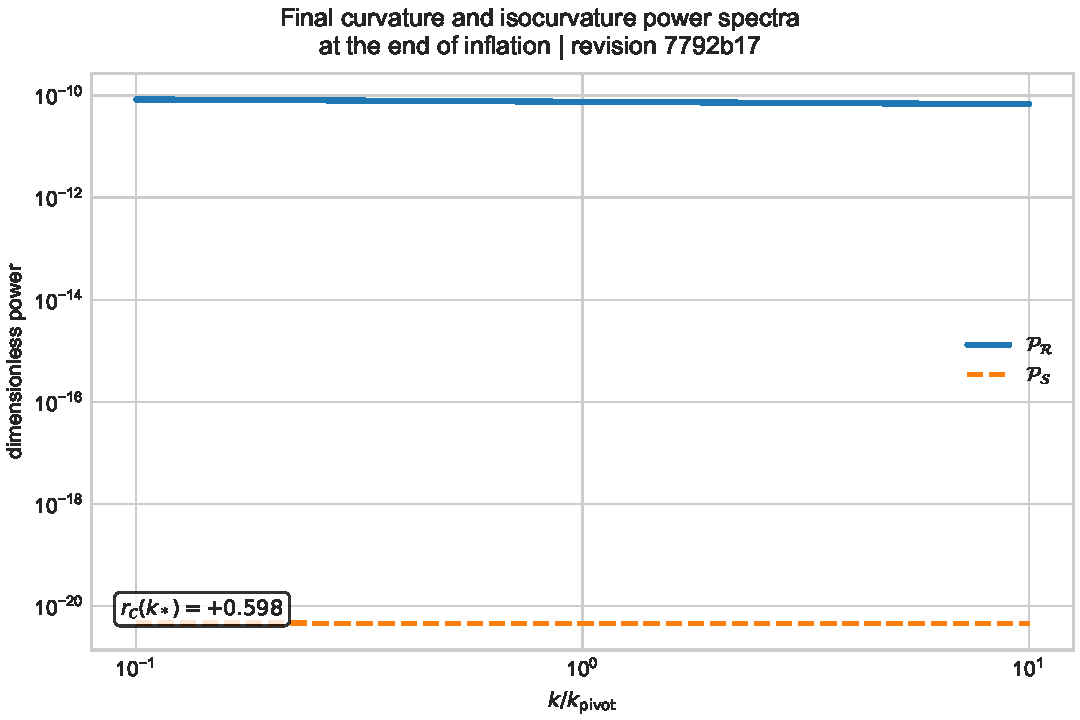
\includegraphics[width=0.95\linewidth]{two_field_final_spectra.pdf}
\caption{最初の科学的マイルストーン：回転のある二場の模型での $\mathcal P_{\mathcal R}$、$\mathcal P_{\mathcal S}$、$\mathcal C_{\mathcal{RS}}$（\repofig{two_field_final_spectra}{two\_field\_final\_spectra}）。}
\end{figure}

%======================================================================
\section{transport とは何か}
\label{sec:transport}
%======================================================================

\subsection{何を計算したいのか}

観測と比べるのは、$\zeta$ の相関関数である。
\[
\langle\zeta_{\mathbf k_1}\zeta_{\mathbf k_2}\rangle=(2\pi)^3\delta^3(\mathbf k_1+\mathbf k_2)P_\zeta(k),\qquad
\langle\zeta_{\mathbf k_1}\zeta_{\mathbf k_2}\zeta_{\mathbf k_3}\rangle=(2\pi)^3\delta^3(\textstyle\sum\mathbf k_r)B_\zeta(k_1,k_2,k_3).
\]
$B_\zeta$（バイスペクトル）は、揺らぎがガウス分布からどれだけずれているかを表す。
その大きさを無次元にしたものが $\fnl$ である。
これを計算する方法は、主に三つある。

\begin{center}
\begin{tabular}{p{2.8cm}p{5.6cm}p{5.6cm}}
\toprule
方法 & 中身 & 得失 \\
\midrule
in-in 形式 & 3次の相互作用を時間で積分する（Maldacena の方法\cite{Maldacena2003}） & 厳密だが、三角形ごと・模型ごとに振動する積分を評価する必要がある \\
$\delta N$ 形式 & 地平線を出たあとは、各点が独立な宇宙として進化すると考え、$N(\phi)$ の微分から $\zeta$ を出す & 簡単だが、地平線の中で生じる相互作用と運動量への依存を落とす \\
\textbf{transport} & 相関関数そのものの常微分方程式を、地平線の内側から外まで解く & 厳密（tree level）で、どんな模型にも同じコードが使える。このリポジトリの方式 \\
\bottomrule
\end{tabular}
\end{center}

\begin{keypoint}[transport の一言での説明]
揺らぎ $X$ の運動方程式から、\textbf{相関関数 $\langle XX\rangle$, $\langle XXX\rangle$ の運動方程式}を直接作り、それを解く。
揺らぎ一つ一つの解（モード関数）を求めてから掛け合わせるのではなく、\emph{平均を取ったあとの量を直接発展させる}。
\end{keypoint}
transport は Mulryne\cite{Mulryne2013} が導入し、Dias--Frazer--Seery\cite{DFS2015}、Dias--Frazer--Mulryne--Seery（DFMS）\cite{DFMS2016}、Butchers--Seery\cite{BS2018} が曲がった場空間へ広げた。
共変な定式化は Gong--Tanaka\cite{GongTanaka2011} と Elliston--Seery--Tavakol\cite{EST2012} による。

\subsection{一次元の toy model}

減衰のある調和振動子を例にする。
\[
\dot q=p,\qquad \dot p=-\gamma p-\omega^2q .
\]
位相空間のベクトル $X=(q,p)^T$ を使うと、
\[
\dot X^a=u^a{}_bX^b,\qquad u=\begin{pmatrix}0&1\\-\omega^2&-\gamma\end{pmatrix}
\]
と書ける。
共分散 $\Sigma^{ab}=\langle X^aX^b\rangle$ の時間微分は、積の微分そのものである。
\[
\dot\Sigma^{ab}=\langle\dot X^aX^b\rangle+\langle X^a\dot X^b\rangle=u^a{}_c\Sigma^{cb}+u^b{}_c\Sigma^{ac},
\qquad\text{つまり}\quad\dot\Sigma=u\Sigma+\Sigma u^T .
\]
これが\textbf{二点の transport 方程式}である。
初期の $\Sigma$（量子論では真空のゆらぎ $\langle q^2\rangle=1/2\omega$ など）を与えれば、あとは $\Sigma$ の三成分（$qq$, $qp$, $pp$）を解くだけで、解 $q(t)$ を経由する必要はない。
量子論では $\langle qp\rangle\neq\langle pq\rangle$ で、その差 $\langle[q,p]\rangle=i$ も保存されるので、$\Sigma$ は複素数として、添字を対称化せずに持つ。

\paragraph{非線形にすると三点関数が出る。}
運動方程式に 2次の項を加える。
\[
\dot X^a=u^a{}_bX^b+\tfrac12u^a{}_{bc}X^bX^c .
\]
三点関数 $\alpha^{abc}=\langle X^aX^bX^c\rangle$ を微分すると
\[
\dot\alpha^{abc}=u^a{}_d\alpha^{dbc}+u^b{}_d\alpha^{adc}+u^c{}_d\alpha^{abd}
+\tfrac12u^a{}_{de}\langle X^dX^eX^bX^c\rangle+(\text{$b,c$ についても同様})
\]
となる。
4点の平均を Wick の定理で二点関数の積に分解すると（tree level ではこれで閉じる）、
$\langle X^dX^eX^bX^c\rangle\to\Sigma^{db}\Sigma^{ec}+\Sigma^{dc}\Sigma^{eb}$ になる。
$u^a{}_{de}$ は $d,e$ について対称なので、二つの項は等しく、$\tfrac12$ が消える。
\begin{equation}
\dot\alpha^{abc}=\underbrace{u^a{}_d\alpha^{dbc}+u^b{}_d\alpha^{adc}+u^c{}_d\alpha^{abd}}_{\text{斉次部分：線形の流れで運ぶ}}
+\underbrace{u^a{}_{de}\Sigma^{db}\Sigma^{ec}+u^b{}_{de}\Sigma^{ad}\Sigma^{ec}+u^c{}_{de}\Sigma^{ad}\Sigma^{be}}_{\text{源：二点関数から三点関数を作る}} .
\label{eq:toy3}
\end{equation}
\textbf{ガウス分布の揺らぎ（$\alpha=0$）から出発しても、源の項によって非ガウス性が生まれ、斉次の項によって運ばれていく。}
これが三点の transport の全体である。

\begin{caution}[演算子の順序]
量子論では、$\Sigma^{ad}$ と $\Sigma^{da}$ は複素共役の関係にあり、等しくない（虚部が交換子にあたる）。
2次の挿入より\emph{左}にある足は $\Sigma^{ad}$、\emph{右}にある足は $\Sigma^{db}$ と、順序を保って縮約しなければならない。
これは DFMS の Eq.~(5.14)\cite{DFMS2016} と一致する。
以前の版ではこれを間違えていて、de Sitter での整合性テストが $O(1)$ ずれた（付録~\ref{app:discrepancies} の 5）。
\end{caution}

\subsection{インフレーションでの transport}

toy model の $q,p$ を、多場の揺らぎに置き換える。
\[
X^a=(Q^I,P^I),\qquad P^I=\Dt Q^I,\qquad \DN\equiv H^{-1}\Dt\ (\text{e-fold で測った共変微分}).
\]
式\eqref{eq:linear}から、線形の流れは
\begin{gather}
\DN Q^I=\frac{P^I}{H},\qquad \DN P^I=-3P^I-\frac{1}{H}\Big(C^I{}_J+\frac{k^2}{a^2}\delta^I{}_J\Big)Q^J,
\notag\\
\Longleftrightarrow\quad
u^a{}_b(k)=\begin{pmatrix}0&H^{-1}\delta^I{}_J\\[2pt]-H^{-1}\big(C^I{}_J+\frac{k^2}{a^2}\delta^I{}_J\big)&-3\delta^I{}_J\end{pmatrix}
\label{eq:u}
\end{gather}
となる。
toy model との違いは三つある。
\begin{enumerate}
\item 係数が時間に依存する（背景の軌道から読む）。背景は一度だけ解いて保存し、三次エルミート補間で読む。
\item 添字が場空間の添字なので、微分は共変微分である。実装では座標微分に、接続による流れ $\Gamma^I{}_{JK}\dot\phi^J/H$ を加える。
\item 三点関数では、三本の足がそれぞれ別の波数 $k_1,k_2,k_3$ を持つ。$u^a{}_b(k_r)$ は足ごとに違い、$u^a{}_{bc}$ は三角形の形（$\mathbf k_i\cdot\mathbf k_j$）に依存する。
\end{enumerate}

\paragraph{二点の transport と検証。}
\[
\DN\Sigma^{ab}(k)=u^a{}_c(k)\Sigma^{cb}(k)+u^b{}_c(k)\Sigma^{ac}(k).
\]
これが正しいことは、独立に作ったモードソルバー（\S\ref{sec:pipeline}）の結果 $\Sigma^{IJ}=\sum_AU^I{}_AU^{J*}{}_A$ と照合して確かめた。
$QQ,QP,PQ,PP$ の四つのブロックすべてが、地平線の中・地平線を出るとき・回転の最中・最後のスライスで $2\times10^{-7}$ 以内で一致する（P3c。モード解から共分散への変換は付録~\ref{app:oracle}）。

\paragraph{三点の transport。}
式\eqref{eq:toy3}の運動量の引数を明示すると
\begin{align}
\DN\alpha^{abc}={}&u^a{}_d(k_1)\alpha^{dbc}+u^b{}_d(k_2)\alpha^{adc}+u^c{}_d(k_3)\alpha^{abd}\notag\\
&+u^a{}_{de}(\mathbf k_1;\mathbf k_2,\mathbf k_3)\Sigma^{db}(k_2)\Sigma^{ec}(k_3)
+u^b{}_{de}(\mathbf k_2;\mathbf k_1,\mathbf k_3)\Sigma^{ad}(k_1)\Sigma^{ec}(k_3)\notag\\
&+u^c{}_{de}(\mathbf k_3;\mathbf k_1,\mathbf k_2)\Sigma^{ad}(k_1)\Sigma^{be}(k_2)
\end{align}
となる。
三つの $\Sigma(k_r)$ と $\alpha$ を同時に発展させる（P3d、実装は \repo{crates/phys-type/src/transport.rs}）。

\subsection{2次の流れ \texorpdfstring{$u^a{}_{bc}$}{u\^{}a\_bc} は 3次の作用から来る}
\label{sec:canonical}

$u^a{}_{bc}$ は、平坦ゲージでの 3次の作用\cite{BS2018}から決まる（Eqs.~(2.9)--(2.15)。係数の全式は付録~\ref{app:cubic}）。
\[
S^{(3)}=\frac12\int dt\,a^3\Big\{A_{IJK}Q^IQ^JQ^K+B_{IJK}Q^IQ^J\Dt Q^K+C_{IJK}\Dt Q^I\Dt Q^JQ^K\Big\}.
\]
係数の一部を抜き出すと、
\[
\widetilde A_{IJK}\ni-\tfrac13V_{;IJK}-\frac{\dot\phi_IV_{;JK}}{2H\Mpl^2}
-\frac{\dot\phi_K\dot\phi^L\dot\phi^M}{2H\Mpl^2}R_{L(IJ)M}+\tfrac13R_{(I|LM|J;K)}\dot\phi^L\dot\phi^M
+\frac{\dot\phi_IG_{JK}}{2H\Mpl^2}\frac{\mathbf k_2\cdot\mathbf k_3}{a^2}+\cdots
\]
のように、ポテンシャルの 3階微分、\textbf{場空間の曲率とその共変微分}、運動量の内積が入る。
P3b で 3階の自動微分と $\nabla R$ を先に実装したのは、このためである。
添字を対称化するときは、添字についているフーリエ運動量も一緒に入れ替えなければならない。

\paragraph{速度と正準運動量。}
ハミルトン形式の導出では、正準運動量 $\Pi_I=a^{-3}\partial\mathcal L/\partial(\Dt Q^I)$ を使う。
3次の作用があると
\[
\Pi_I=\Dt Q_I+\tfrac12B_{JKI}Q^JQ^K+C_{IJK}\Pi^JQ^K+O(Q^3)
\]
となり、線形では一致するが \emph{2次でずれる}。
三点関数はちょうどこの次数で効く。
そこで発展は正準の基底 $(Q,\Pi)$ で行い、速度の基底へは名前の付いた変換関数でだけ移れるようにした。
二つの基底を混ぜたコードは、コンパイル失敗テスト \code{mix\_velocity\_and\_canonical\_phase\_space} が示すとおり通らない。

\subsection{初期条件}

三点関数の初期値を $\alpha=0$ にするのは誤りである。
地平線を出る前後の相互作用で生じる寄与を落としてしまうからである。
実装では、地平線の十分内側の共通のスライスで、Bunch--Davies 真空に 3次の相互作用を一次まで入れた tree level の値を、8 ブロックすべてに与える。
三本の足のうち、いちばん短い波数が $k/aH=e^{\Delta N}$ になる時刻を開始時刻にする。
開始を深くしたときの収束は $x_{\rm init}^{-1}$ のように進み、許容誤差についても収束を確かめた。
非線形な場の再定義のもとで、テンソルとして変換することも $4\times10^{-10}$ で確かめた。

\subsection{\texorpdfstring{$\zeta$}{ζ} への射影}
\label{sec:projection}

最後に、地平線の外のスライスで、場の揺らぎを曲率摂動 $\zeta$ に 2次まで変換する（Dias ほか\cite{DEFMS2015}の ``simple'' 表示、実装は \repo{crates/phys-type/src/curvature.rs}。全式は付録~\ref{app:gauge}）。
\[
\zeta=N_aX^a+\tfrac12N_{ab}X^aX^b,\qquad N_I=-\frac{\dot\phi_I}{2H\Mpl^2\epsilon}\quad(\text{線形では }\zeta=-\mathcal R),
\]
\begin{equation}
P_\zeta=N_IN_J\,\mathrm{Re}\,\Sigma^{IJ}_{QQ},\qquad
B_\zeta=\underbrace{N_IN_JN_K\alpha^{IJK}_{QQQ}}_{\text{intrinsic}}
+\underbrace{\sum_rN_aN_bN_{cd}\Sigma^{ac}\Sigma^{bd}}_{\text{ゲージ変換の寄与}} .
\end{equation}
$\fnl$ は Maldacena\cite{Maldacena2003} と Planck\cite{Planck2018X} の規約で
\begin{equation}
B_\zeta=\frac65\fnl\big[P_\zeta(k_1)P_\zeta(k_2)+P_\zeta(k_1)P_\zeta(k_3)+P_\zeta(k_2)P_\zeta(k_3)\big]
\end{equation}
と定める。
この符号の規約だと、単一場の squeezed 極限で $\fnl\to\tfrac5{12}(1-n_s)>0$ となる。
$N_{Q\Pi}$ の係数は、DFMS の Eq.~(7.4b)\cite{DFMS2016} の $1/3$ ではなく $1/6$ が正しい。
$1/3$ のままだと Maldacena の結果と合わず、$\zeta$ も保存しない（付録~\ref{app:discrepancies} の 1）。

\subsection{\texorpdfstring{$\delta N$}{δN} との関係}

$\delta N$ 形式では、初期スライスで場を $\delta\phi$ だけずらし、終わりの一様密度面までの e-fold 数 $N(\phi)$ の変化を $\zeta$ とみなす。
\[
\zeta=N_{,a}\delta\phi^a+\tfrac12N_{;ab}\delta\phi^a\delta\phi^b,\qquad
\frac65\fnl^{\delta N}=\frac{N_{,a}N_{,b}N^{;ab}}{(N_{,c}N^{,c})^2}.
\]
\begin{itemize}
\item \textbf{crossing-time $\delta N$}：地平線を出たときの場の値で微分し、速度は slow roll の値に固定する（KMS の方法）。地平線の中の相互作用と、速度の揺らぎを落とす。
\item \textbf{phase-space $\delta N$}：地平線を出た数 e-fold 後のスライスで、場と速度の両方を（固有時の速度で）ずらす。transport と $10^{-4}$ 程度で一致するので、独立な検算に使える。
\end{itemize}

\subsection{transport の検証一覧}

\begin{center}
\small
\begin{tabular}{p{6.2cm}p{7.4cm}}
\toprule
検証 & 結果 \\
\midrule
二点 transport とモードソルバー & 4 ブロックすべてで $2\times10^{-7}$ \\
$P_\zeta$ とモードソルバーの $\mathcal P_{\mathcal R}$ & 相対誤差 $6\times10^{-9}$ \\
単一場での Maldacena の結果 & 1.7〜3.6\%（slow roll の次の次数の差） \\
squeezed の整合性関係 $\tfrac5{12}(1-n_s)$ & 0.021071 と 0.021001。差は $(k_3/k_1)^2$ で減る \\
axion-quartic 模型\cite{Elliston2012}（DFMS Fig.~7\cite{DFMS2016}） & 曲線全体で一致（例：$-39.2236$ と $-39.2245$） \\
axion-quartic 模型の数値 $\delta N$ & 13.106 と transport の 13.120 \\
3 場の分離型の模型\cite{BattefeldEasther2007} & phase-space $\delta N$ と $2\times10^{-5}$ \\
場の再定義（剪断した座標） & $P_\zeta$ が $10^{-8}$、$B_\zeta$ が $10^{-7}$ で不変 \\
constant turn での bispectrum の振幅\cite{HMPS2026b} & in-in の独立計算と $10^{-5}$ \\
\bottomrule
\end{tabular}
\end{center}

%======================================================================
\section{KMS：二場がともに非最小結合する模型}
\label{sec:kms}
%======================================================================

\subsection{なぜこの模型か}

これまでに検証した非最小結合の模型（Higgs inflation\cite{BezrukovShaposhnikov2008}、nonminimally assisted inflation\cite{HKKPT2023}）では、$\Omega^2$ が一つの場にしか依存しなかった。
その場合、Einstein frame の計量は一つの座標の関数で、二場の曲率も $K(s)$ という一変数の関数になる。
KMS は\textbf{二つの場がともに $R$ に結合する}模型で、計量は非対角になり、等長変換もない。
曲率は方向ごとに変わる。
transport の曲率の項（質量行列の Riemann テンソルと、3次の係数に入る $\nabla R$）が大きく効く、一般的な状況をテストできる。
コードは \repo{crates/phys-type-models/src/kms.rs} にある。

\subsection{模型}

Kaiser, Mazenc, Sfakianakis\cite{KMS2013}（以下 [KMS]）の Eqs.~(16)--(17)。
\[
f(\phi,\chi)=\tfrac12\big[\Mpl^2+\xi_\phi\phi^2+\xi_\chi\chi^2\big],\qquad
\tilde V=\tfrac{\lambda_\phi}4\phi^4+\tfrac g2\phi^2\chi^2+\tfrac{\lambda_\chi}4\chi^4\quad(m_\phi=m_\chi=0).
\]
式\eqref{eq:jordan}の記法では $\Omega^2=1+\xi_\phi\phi^2+\xi_\chi\chi^2$（$\Mpl=1$）、$k_{IJ}=\delta_{IJ}$、$V_J=\tilde V$ である。
ベンチマークのパラメータは
\[
\xi_\phi=10,\quad\xi_\chi=10.02,\quad\lambda_\chi/\lambda_\phi=0.5,\quad g/\lambda_\phi=1,\quad\phi(\tau_0)=3.1\,\Mpl .
\]
$\lambda_\phi$ は振幅を決めるだけなので、形に関する観測量は $\lambda_\phi$ によらない（コードでは $10^{-2}$）。

\paragraph{尾根と谷。}
場の値が大きいとき、Einstein frame のポテンシャルは
\[
V\to\frac{\Mpl^4}{4}\frac{\lambda_\phi\phi^4+2g\phi^2\chi^2+\lambda_\chi\chi^4}{(\xi_\phi\phi^2+\xi_\chi\chi^2)^2}
\]
となる。
$\phi$ 軸上の値 $\lambda_\phi/\xi_\phi^2$ は、$\chi$ 軸上の値 $\lambda_\chi/\xi_\chi^2$ の約 2 倍なので、\textbf{$\chi=0$ は尾根}である。
三本の軌道は尾根の上の、尾根から少しだけ離れた点から出発する。
尾根から落ちる時刻は軌道ごとに違い、落ちたあとは $\chi$ 方向の谷へ曲がっていく。
地形の図と、「尾根」がどういう意味で尾根なのか（素朴に $\phi$ を固定して見ると谷に見える）は、\S\ref{sec:kms-landscape} で説明する。

\begin{center}
\begin{tabular}{cc}
\toprule
軌道 & $\chi(\tau_0)/\Mpl$ \\
\midrule
1 & $1.1\times10^{-2}$ \\
2 & $1.1\times10^{-3}$ \\
3 & $1.1\times10^{-4}$ \\
\bottomrule
\end{tabular}
\end{center}

\subsection{Einstein frame の幾何（G1）}

式\eqref{eq:einstein}に代入すると（$\partial_\phi\Omega^2=2\xi_\phi\phi$ なので、$\kappa$ の項は $\tfrac32\cdot4\xi^2\phi^2/\Omega^4$ になる）、
\begin{equation}
G_{IJ}=\frac{1}{\Omega^2}\begin{pmatrix}1&0\\0&1\end{pmatrix}
+\frac{6\kappa}{\Omega^4}\begin{pmatrix}\xi_\phi^2\phi^2&\xi_\phi\xi_\chi\phi\chi\\\xi_\phi\xi_\chi\phi\chi&\xi_\chi^2\chi^2\end{pmatrix}
\qquad\text{([KMS] Eq.~110\cite{KMS2013}; Kaiser\cite{Kaiser2010})}.
\end{equation}
二次元なので、Riemann テンソルはガウス曲率 $K$ 一つで決まる。
\[
R^I{}_{JKL}=K\big(\delta^I{}_KG_{JL}-\delta^I{}_LG_{JK}\big).
\]
\begin{align}
\text{metric：}&\quad K=\frac{(1+6\xi_\phi)(1+6\xi_\chi)\Omega^4-C^2}{6C^2},\qquad C=\Omega^2+6\xi_\phi^2\phi^2+6\xi_\chi^2\chi^2,\\
\text{Palatini：}&\quad K=\xi_\phi+\xi_\chi-\frac{2(\xi_\phi^2\phi^2+\xi_\chi^2\chi^2)}{\Omega^2}.
\end{align}
自動微分で作った幾何（\code{einstein\_frame}）と、この閉じた式を比べると、計量は $10^{-13}$、Riemann テンソルは $10^{-10}$、$\nabla R$ は差分の誤差の範囲で一致した。
metric と Palatini の両方で、一般のパラメータでも確かめている（\repo{crates/phys-type-models/tests/kms.rs}）。

\begin{caution}[論文の誤植：entry 14]
[KMS] Eq.~(115) は場空間の Ricci スカラー $\mathcal R=2K$ を載せているが、その値は正しい値の\textbf{2倍}になっている（印刷された式は $4K$ に等しい）。
TeX のソースで確かめ、sympy（Brioschi の公式）で独立に計算して確認した（付録~\ref{app:discrepancies} の 14）。
\end{caution}

\subsection{ポテンシャルの地形：ボールが転がる絵で見る}
\label{sec:kms-landscape}

\begin{figure}[!htbp]
\centering
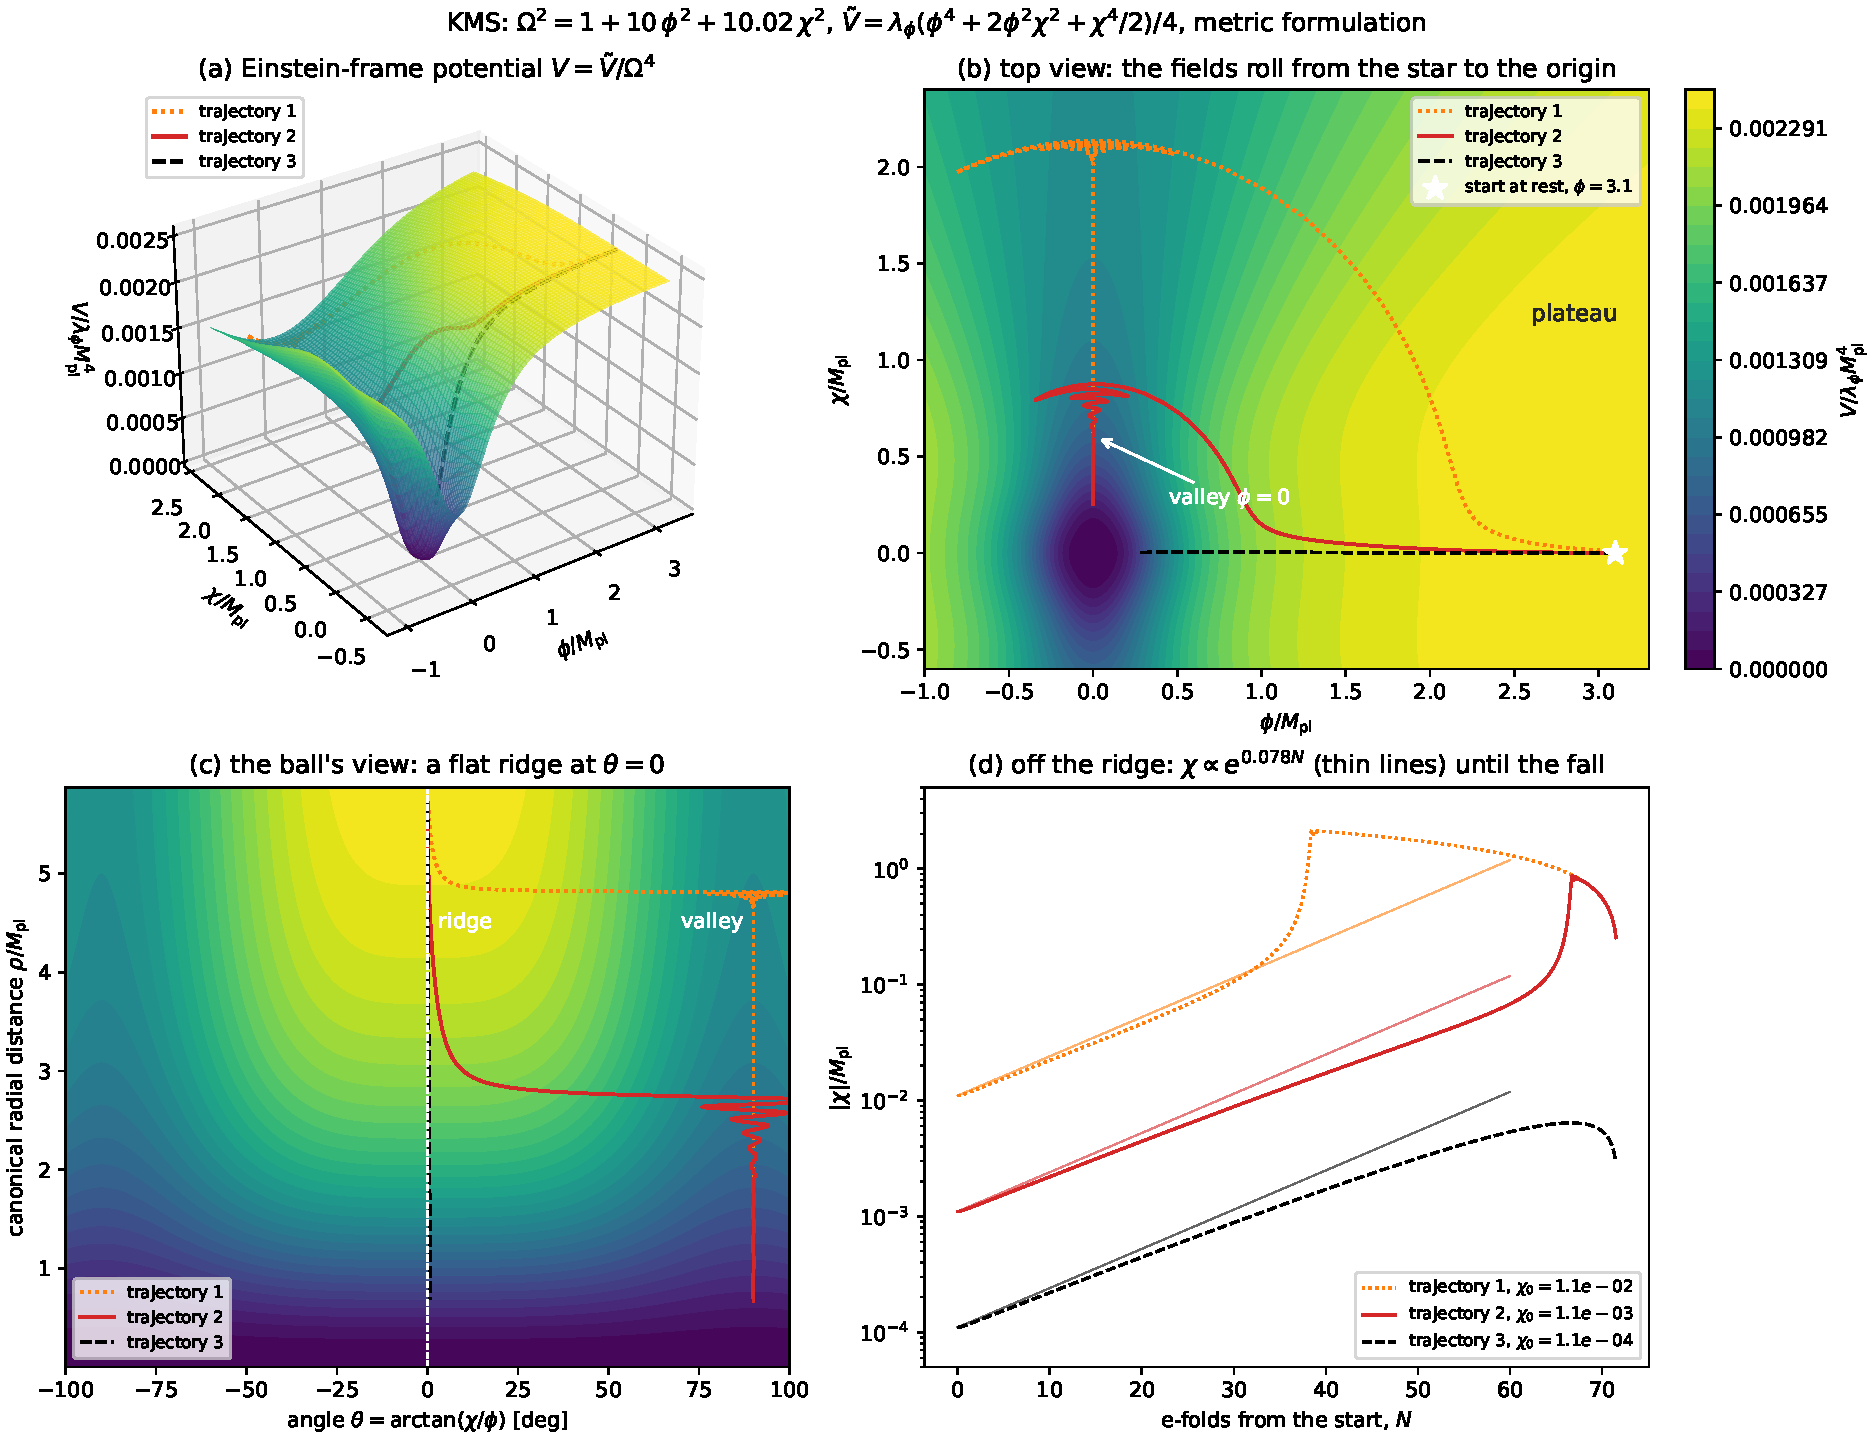
\includegraphics[width=0.97\linewidth]{kms_potential.pdf}
\caption{KMS の Einstein frame でのポテンシャルと三本の軌道（このノートと同じディレクトリの \code{kms\_potential.py}、軌道は \href{\repourl/blob/\reporev/golden/kms_trajectories.csv}{\code{golden/kms\_trajectories.csv}}）。
(a) 作用の座標 $(\phi,\chi)$ で描いた地形。
(b) 真上から見た図。星印から出発し、原点へ転がる。
(c) 場空間がほぼ平らに見える座標（角度 $\theta$ と、正準に規格化した動径 $\rho$）で描いた図。$\theta=0$ に平らな尾根、$\theta=\pm90^\circ$ に谷がある。
(d) 尾根の上で $\chi$ が e-fold あたり一定の割合で増える様子。細線は、共変な質量から見積もった $e^{0.078N}$。}
\label{fig:kms-potential}
\end{figure}

\paragraph{全体の地形。}
場の値が大きいところで $\xi_\phi\approx\xi_\chi\equiv\xi$ とし、極座標 $\phi=r\cos\theta$, $\chi=r\sin\theta$ を使うと、$\Omega^2\approx1+\xi r^2$ はほぼ $r$ だけの関数になる。
$g=\lambda_\phi$, $\lambda_\chi=\lambda_\phi/2$ を代入すると、
\begin{equation}
V\;\xrightarrow{\ \xi r^2\gg1\ }\;\frac{\lambda_\phi\Mpl^4}{4\xi^2}\Big(\cos^4\theta+2\cos^2\theta\sin^2\theta+\tfrac12\sin^4\theta\Big)
=\frac{\lambda_\phi\Mpl^4}{4\xi^2}\Big(1-\tfrac12\sin^4\theta\Big)
\label{eq:kms-angular}
\end{equation}
となる。
\begin{itemize}
\item \textbf{動径方向}には平らな台地（plateau）がある。Higgs inflation と同じで、$\Omega^4$ で割ることで $\phi^4$ が平らになる。
\item \textbf{角度方向}では、$\theta=0$（$\phi$ 軸）が最大で \textbf{尾根}、$\theta=\pm90^\circ$（$\chi$ 軸）が高さ半分の\textbf{谷}になる。
\item 尾根は $1-\tfrac12\theta^4$ のように\textbf{非常に平ら}である。$\xi_\chi=\xi_\phi$ なら尾根を横切る方向の2階微分は厳密に 0 になり、尾根の不安定性は $\xi_\chi-\xi_\phi=0.02$ という小さな差だけから生じる。
\end{itemize}
ボールの絵で言えば、平らな台地の上の、ほとんど平らな尾根の上にボールを置いた状態である。
ボールはごくゆっくり尾根から転がり落ち、谷へ曲がり、谷を下って原点に向かう。

\paragraph{素朴な絵の落とし穴：場空間は曲がっている。}
$\phi$ を固定して $\chi$ の向きに見ると、$\phi=3.1$ で
\[
\partial_\chi^2V\big|_{\chi=0}=+8.5\times10^{-6}\lambda_\phi\Mpl^2>0
\]
となり、$\chi=0$ は\emph{谷}に見えてしまう。
ボールの運動を決めるのは、場空間の計量込みの共変なヘッセ行列である。
\[
V_{;\chi\chi}=V_{,\chi\chi}-\Gamma^\phi{}_{\chi\chi}V_{,\phi},\qquad
\Gamma^\phi{}_{\chi\chi}\simeq\frac1\phi\quad(\text{この模型では }\xi\phi^2\gg1\text{ でほぼ厳密}).
\]
$\Gamma^\phi{}_{\chi\chi}=1/\phi$ は、平らな平面を極座標で書いたときの値と同じである。
つまり $(\phi,\chi)$ は、実質的に「動径と角度」としてふるまう。
そのため $V_{;\chi\chi}$ は角度方向の2階微分 $r^{-2}\partial_\theta^2V$ に等しくなり、符号は\textbf{負}になる。
\begin{center}
\begin{tabular}{ccccc}
\toprule
$\phi$ & $V_{,\chi\chi}$ & $V_{;\chi\chi}$ & $m^2/H^2=G^{\chi\chi}V_{;\chi\chi}/H^2$ & 成長率 $-\tfrac32+\sqrt{\tfrac94-m^2/H^2}$ \\
\midrule
3.1 & $+8.5\times10^{-6}$ & $-2.0\times10^{-6}$ & $-0.24$ & 0.078 \\
2.0 & $+5.3\times10^{-5}$ & $-4.7\times10^{-6}$ & $-0.25$ & 0.079 \\
\bottomrule
\end{tabular}
\end{center}
（単位は $\lambda_\phi=\Mpl=1$。曲率の項と重力の項を除いた、ポテンシャルだけの寄与。）
尾根を横切る方向には $m^2\approx-0.24H^2$ のタキオン的な質量があり、$\chi$ は $e^{0.078N}$ で増える。
実際の軌道で測ると、尾根の上での $d\ln\chi/dN$ は 0.073（軌道 1）、0.068（軌道 2）、0.058（軌道 3）で、見積もりとおおむね合う。
残る差の原因として考えられるのは、ここで除いた曲率の項 $K\dot\sigma^2>0$ などである（まだ確かめていない）。

図\ref{fig:kms-potential}(c) は、場空間がほぼ平らに見える座標（角度 $\theta$ と正準な動径 $\rho=\int\sqrt{G_{rr}}\,dr$）で描いたもので、ボールの絵が正しく成り立つのはこの図である。
ただし、角度方向の固有の長さは $\sqrt{G_{\theta\theta}}\,d\theta=(r/\Omega)\,d\theta\approx d\theta/\sqrt\xi$ である。
したがって、度で描いた横軸は実際の距離を約 $\sqrt{10}\approx3$ 倍に引き伸ばしている。

\paragraph{三本の軌道を定性的に読む。}
尾根から離れる速さが一定なので、$\chi_0$ が 10 倍違う軌道は、$\ln10/0.078\approx30$ e-fold ずれて落ちる。
実測では、軌道 1 と軌道 2 の回転のピークの間隔は 28.9 e-fold である。
以下の解釈は、図から読み取った定性的なものである。
\begin{itemize}
\item \textbf{軌道 1}（$\chi_0=1.1\times10^{-2}$）：台地の奥（$\rho\approx5$）で早めに尾根から落ち、台地の上を横に滑って谷に入る。谷の台地は高さが半分になるだけで、まだ平らなので、そのあと 34 e-fold ほど slow roll が続く。曲がったあとの時間が長いので、終わりの時刻は初期のずれにあまり敏感でなく、$\fnl$ は小さい（0.013）。
\item \textbf{軌道 2}（$\chi_0=1.1\times10^{-3}$）：台地の縁近く（$\rho\approx2.8$）、終わりの約 5 e-fold 前に落ちる。台地の縁は急なので、横に転がり落ちるときに運動エネルギーが大きくなり、$\epsilon_H$ は 0.99 まで上がる。pivot のモード（end の 60 e-fold 前に地平線を出たもの）はすでに地平線の外にあり、曲がり角で等曲率摂動が曲率摂動に変わる。終わりの時刻が初期のずれに非線形に強く依存するので、$\fnl$ は大きい（43）。
\item \textbf{軌道 3}（$\chi_0=1.1\times10^{-4}$）：落ちる前にインフレーションが終わる。ずっと尾根の上を進む単一場の運動なので、$\fnl$ は小さい。
\end{itemize}

\subsection{背景の三本の軌道（G2）}

\begin{center}
\begin{tabular}{lcc}
\toprule
量 & このリポジトリ & [KMS] \\
\midrule
軌道 2 の総 e-fold 数（静止から出発） & 71.517 & 71.5（Fig.~3） \\
軌道 2 の総 e-fold 数（slow roll の速度から出発） & 71.19 & --- \\
回転率の最初の山（軌道 1、end の何 e-fold 前か） & 34.06 & 34.5（Fig.~7） \\
回転率の最初の山（軌道 2） & 5.15 & 4.9 \\
二つの山の間隔 & 28.9 & 29.6 \\
軌道 3 & 尾根の上のまま終わる & 同じ \\
\bottomrule
\end{tabular}
\end{center}
総 e-fold 数から、[KMS] は\textbf{静止した状態から出発している}と読み取れる。
論文には書かれていないが、slow roll の速度から出発すると 71.19 になり、合わない。
回転率 $|\eta_\perp|$ は、尾根から落ちるときに最初の山（$\simeq0.8$ と $1.7$）を作る。
そのあと $\phi$ が谷の中で振動するので、$10^2$〜$10^3$ のスパイクが立つ。
Fig.~7 のピークに対応するのは最初の山のほうである。

\subsection{軌道 2 ではインフレーションが止まりかける}

\begin{keypoint}[図を作って見つかったこと]
軌道 2 では、曲がり角で $\epsilon_H$ が \textbf{0.990} まで上がる（軌道 1 は 0.954）。
$6.9\times10^{-4}\lesssim\chi(\tau_0)\lesssim1.0\times10^{-3}$ の範囲では実際に $\epsilon_H=1$ に届き、計算はそこで終わる。
総 e-fold 数は 67.8〜71.4 に下がる。
そのとき場はまだ谷の中にあり（$\chi\simeq0.5$〜$0.8$）、物理的にはそのあともインフレーションが続く。

[KMS] の大きな $|\fnl|$ は、この範囲のすぐ外側にある。
crossing-time $\delta N$ は、$\chi(\tau_0)=1.05\times10^{-3}$ で $+2\times10^2$、$6.3\times10^{-4}$ で $-1.6\times10^3$ まで振れる。
[KMS] が「初期条件のわずかな違いで劇的に変わる」と書いている理由は、インフレーションが一度止まりかけることにある。
その結果、値はインフレーションの終わりをどう定義するかにも左右される。
\end{keypoint}

\begin{figure}[t]
\centering
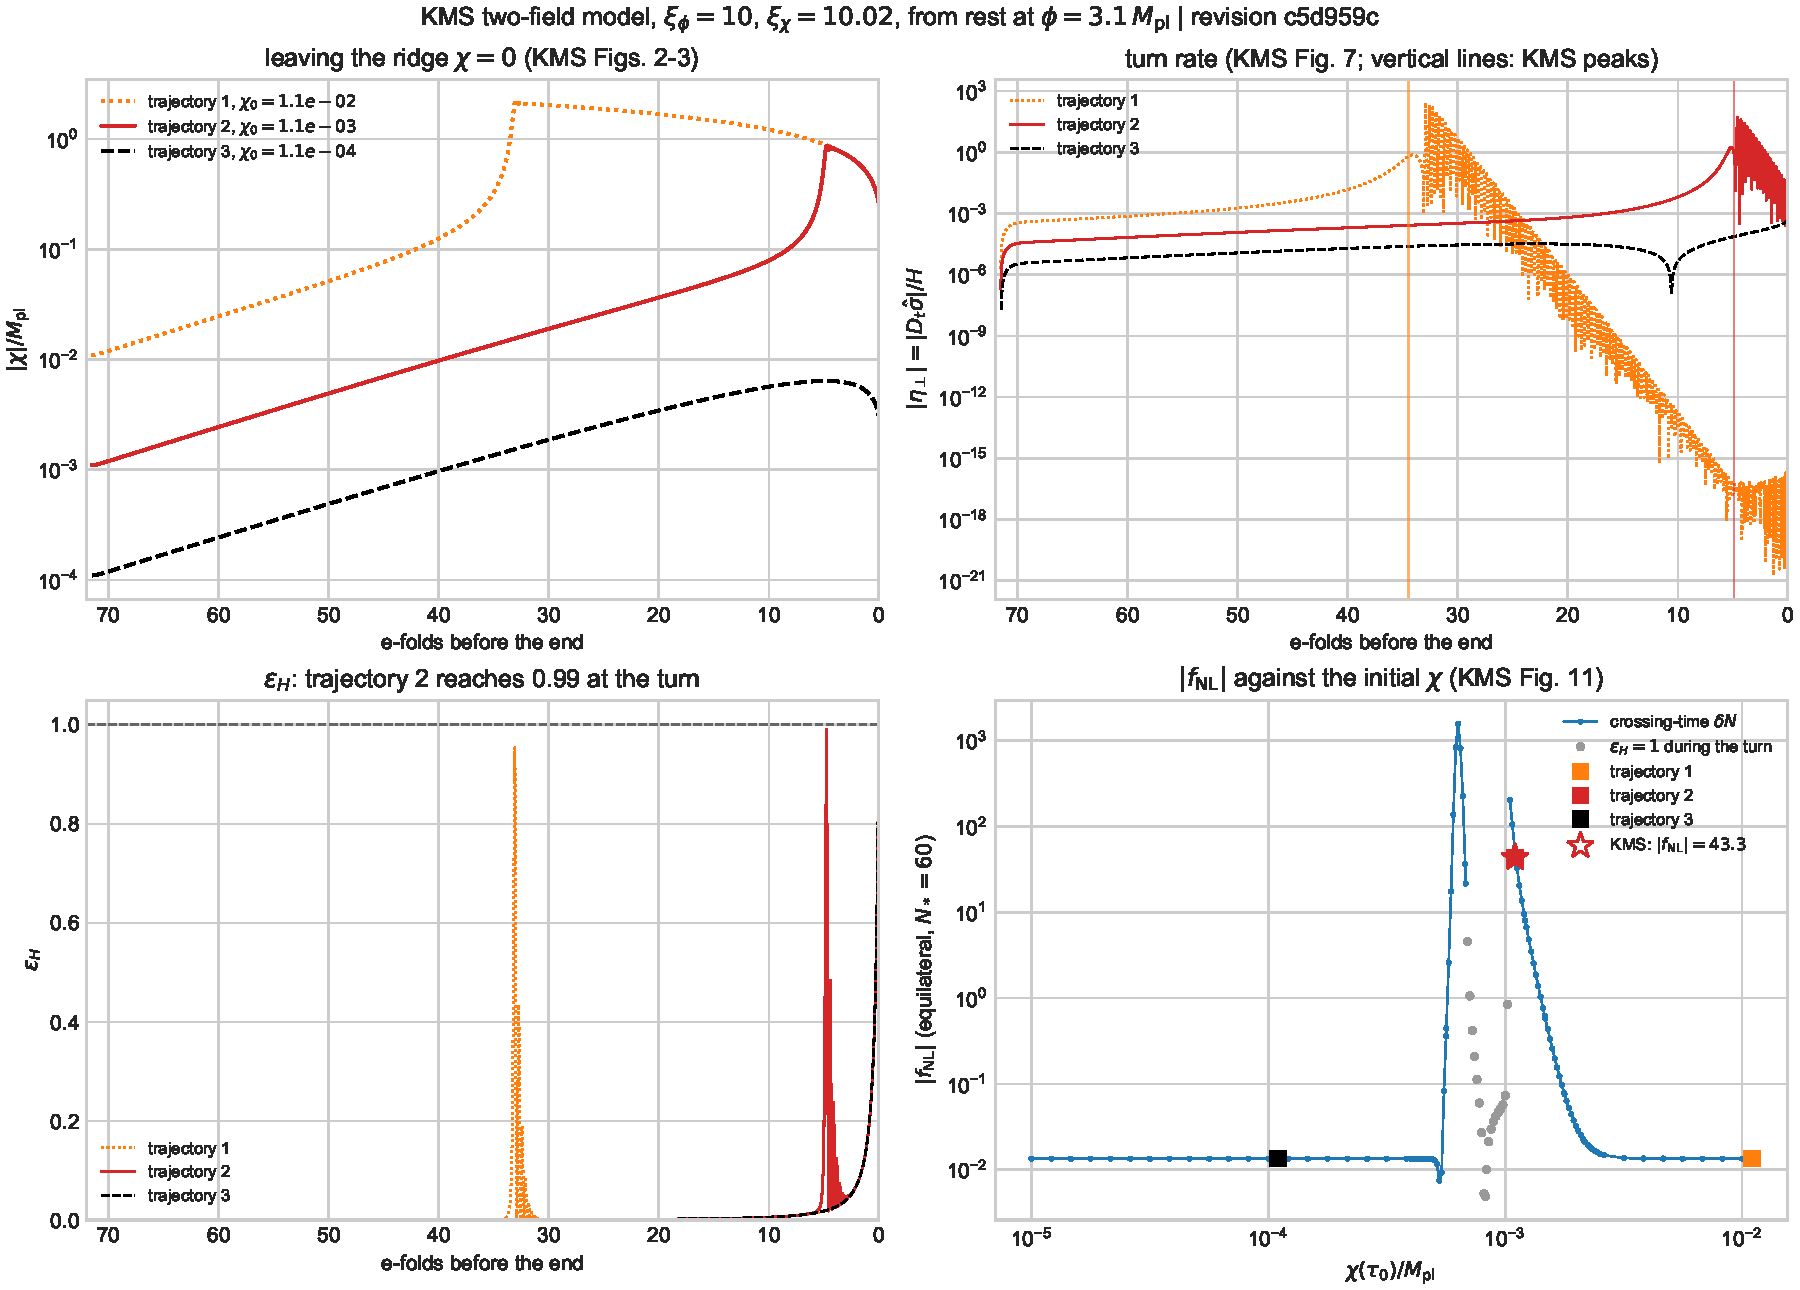
\includegraphics[width=\linewidth]{kms_trajectories.pdf}
\caption{KMS の三本の軌道（\repofig{kms_trajectories}{kms\_trajectories}）。
左上：尾根 $\chi=0$ から $\chi$ が指数的に離れていく様子（[KMS] Figs.~2--3）。
右上：回転率 $|\eta_\perp|$。縦線は [KMS] Fig.~7 のピーク。
左下：$\epsilon_H$。軌道 2 は曲がり角で 0.99 に達する。
右下：crossing-time $\delta N$ による $|\fnl|$ を $\chi(\tau_0)$ に対して描いたもの（[KMS] Fig.~11）。灰色は曲がり角で $\epsilon_H=1$ に届いた点、星印は [KMS] の 43.3。}
\end{figure}

\subsection{\texorpdfstring{$\fnl$：crossing-time $\delta N$}{fNL：crossing-time δN}（G4、KMS の方法）}

[KMS] と同じ方法（pivot は $N_*=60$、地平線を出たときの場の値で中心差分、速度は slow roll、Riemann の項は落とす）で計算した。
\begin{center}
\begin{tabular}{lcc}
\toprule
 & このリポジトリ & [KMS] \\
\midrule
軌道 2 の $|\fnl|$ & 43.38 & 43.3 \\
軌道 1・3 の $|\fnl|$ & 0.013 & 無視できる \\
$P_\zeta$ と厳密なモードソルバー & 5\% 低い（slow roll の速度による） & --- \\
\bottomrule
\end{tabular}
\end{center}
刻み幅を変えても $10^{-3}$ の範囲で安定している（テストは \repo{crates/phys-type-models/tests/kms_trajectories.rs}）。
このリポジトリの規約では符号は正になる（[KMS] Eq.~(92) は逆の符号）。

\subsection{\texorpdfstring{$\fnl$}{fNL}：transport（G4、未解決）}

\begin{caution}[transport が収束しない]
軌道 2 では、tree level の transport の $\fnl$ が\textbf{許容誤差に比例して変わる}。
\begin{center}
\begin{tabular}{cc}
\toprule
相対許容誤差 & transport の $\fnl$ \\
\midrule
$10^{-11}$ & $-6\times10^4$ \\
$10^{-12}$ & $-6\times10^3$ \\
$10^{-13}$ & $-670$ \\
\bottomrule
\end{tabular}
\end{center}
\begin{itemize}
\item すべて intrinsic の項 $N_aN_bN_c\alpha^{abc}$ から来ている。
\item 背景の許容誤差と、開始の深さには依存しない。
\item 線形の部分（$P_\zeta$, $n_s$）は、許容誤差が $10^{-11}$ 以下ならモードソルバーと一致する。
\item 回転の最中に $P_\zeta$ は最終値 $7.2\times10^{-4}$ の $5\times10^5$ 倍まで成長し、等曲率摂動が減衰すると打ち消し合って小さくなる。
\end{itemize}
\end{caution}

\paragraph{解釈（仮説）。}
最終的な三点関数は、途中の巨大な相関関数どうしが打ち消し合った小さな\emph{残り}である。
相対許容誤差 $\varepsilon$ で積分すると、途中の大きさに比例した誤差 $\sim\varepsilon\times(\text{途中の最大値})$ が残る。
誤差が $\varepsilon$ に比例するという観測は、この見方と合っている。
ただし、どこで精度が失われるかはまだ特定していない。
候補は、鋭い回転（$\eta_\perp\simeq50$）か、そのあとの谷での $\phi$ の激しい振動である。

\paragraph{次の手。}
\begin{enumerate}
\item 精度が失われる場所を特定する（区間ごとに許容誤差を変えて比べる）。
\item 条件のよい基底で発展させる（たとえば運動学的基底 $(\sigma,s)$ や、規格化を変えた変数）。
\item 残りがまだ小さくならないスライスで transport を終え、そこからは phase-space $\delta N$ でつなぐ。
\item 独立な参照として、KMS で phase-space $\delta N$ を実際に計算する（まだ実行していない）。
\end{enumerate}
解決するまでは、この模型で transport が検証されたとは言えない。
G4 の参照は $\delta N$ である。

\subsection{KMS の残り}

\begin{center}
\begin{tabular}{lll}
\toprule
段階 & 状態 & 内容 \\
\midrule
G1 & 完了 & 幾何の閉じた式と自動微分の一致。Eq.~115 の誤植を発見 \\
G2 & 完了 & 三本の軌道、図、インフレーションの中断に近いことの発見 \\
G3 & 未着手 & $n_s$（[KMS] は 0.967）と $T_{\mathcal{RS}}$。軌道 2 の終わりでの厳密な $n_s$ は 0.936 \\
G4 & 一部完了 & crossing-time $\delta N$ は一致。transport は収束しない \\
G5 & 未着手 & Palatini 版。比べられる文献値がないので整合性のチェックだけ \\
G6 & 範囲外 & Jordan frame の $\zeta$。別に設計する \\
\bottomrule
\end{tabular}
\end{center}
G3 の注意：[KMS] の $n_s=0.967$ は地平線を出たときの値で、終わりで評価した厳密な値（0.936）とは定義が違う。

%======================================================================
\section{その他の再現結果}
%======================================================================

\begin{center}
\small
\begin{tabular}{p{4.2cm}p{9.4cm}}
\toprule
対象 & 結果 \\
\midrule
二場の背景と線形摂動 & 二つの時間変数の定式化が $3.1\times10^{-10}$ で一致 \\
nonminimally assisted inflation\cite{HKKPT2023} & loop・power-law・hybrid を再現。式 (3.1) と厳密な $n_s$ が $1.5\times10^{-3}$。transport の $\fnl$ を phase-space $\delta N$ で確認。誤植など（entries 6--9, 11） \\
厳密な constant-turn 解\cite{HMPS2026} & 強い混合のスペクトルが $3.5\times10^{-4}$。Eq.~(39) の対数に誤植（entry 10） \\
constant turn での bispectrum\cite{HMPS2026b} & 振幅が $10^{-5}$ で一致。squeezed の閉じた式の前因子は $10/9$ 倍が必要（entry 12）。弱い混合の極限で準単一場\cite{ChenWang2010}の係数を再現 \\
Higgs inflation\cite{BezrukovShaposhnikov2008,BauerDemir2008}（metric / Palatini） & $\xi$ に対する $n_s$ と $r$。Planck\cite{Planck2018X} の等高線に重ねた図（フィットではない） \\
3 場 & 分離型の模型\cite{BattefeldEasther2007}で、phase-space $\delta N$ と $2\times10^{-5}$ \\
\bottomrule
\end{tabular}
\end{center}

%======================================================================
\section{現状のまとめ}
%======================================================================

\begin{center}
\small
\begin{tabular}{lll}
\toprule
機能 & 状態 & 補足 \\
\midrule
型による物理チェック & 完了 & コンパイル失敗テスト 25 件 \\
背景と線形摂動（$N$ 場） & 完了 & $P_\zeta, n_s, r$、等曲率・相互相関 \\
二点 transport & 完了 & モードソルバーと一致 \\
三点 transport と $\fnl$ & 完了 & tree level、インフレーション中のみ、再加熱なし \\
非最小結合の理論から Einstein frame & 完了 & metric と Palatini \\
KMS & 途中 & transport の収束が未解決 \\
\bottomrule
\end{tabular}
\end{center}
テストは、コアのユニットテストが 238 件、models のテストが 17 件と KMS の分、コンパイル失敗が 25 件である。
重いテスト（release モードで \code{--ignored} を付けて手元で実行し、CI では走らない）が 30 件と KMS の 2 件ある。
適用範囲の外にあるもの：ループ補正、再加熱とインフレーション後の発展（遅い時期の等曲率摂動\cite{SSK2014}を含む）、Horndeski と DHOST\cite{ZGB2014,LangloisNoui2016,BLN2016}、Jordan frame の $\zeta$\cite{WMS2012}。
\appendix

%----------------------------------------------------------------------
\section{フレームの対応}
\label{app:frames}
%----------------------------------------------------------------------

$g^E_{\mu\nu}=\Omega^2g^J_{\mu\nu}$ を平坦な FRW 背景に適用すると、$dt_E=\Omega\,dt_J$、$a_E=\Omega\,a_J$ となる。
場の座標は両方のフレームで共通で、変わるのは計量と時間座標だけである。
Einstein frame の状態から、Jordan frame の量は次のように求まる（\code{EinsteinFrame::correspondence}）。
\begin{center}
\begin{tabular}{ll}
\toprule
Jordan frame の量 & 式（ドットは $d/dt_E$） \\
\midrule
スケール因子 & $a_J=a_E/\Omega$ \\
e-fold 数 & $N_J=N_E-\ln\Omega$ \\
Hubble 率 & $H_J=\Omega\left(H_E-\dot\phi^I\partial_I\ln\Omega\right)$ \\
場の速度 & $d\phi^I/dt_J=\Omega\,\dot\phi^I$ \\
ポテンシャル & $V_J=\Omega^4V$ \\
\bottomrule
\end{tabular}
\end{center}

\paragraph{e-fold 数はフレームに依存し、物理的な波数での観測量は依存しない。}
区間の長さは $\Delta N_J=\Delta N_E-\Delta\ln\Omega$ だけ違う。
したがって「pivot が end の 60 e-fold 前に地平線を出る」と言ったとき、二つのフレームでは別の物理スケールを指す。
単一場では $\zeta$ がフレームによらず、インフレーションの後は $\Omega\to1$ なので、物理的な波数 $k$ を固定した $n_s(k)$ はフレームによらない。
変わるのはラベルだけである。
Higgs inflation では pivot から end までの区間が約 1.8 e-fold 違い、「$N_*=60$」が指すスケールの $n_s$ は $10^{-3}$ ほど違う。
Palatini Higgs inflation の $\xi=10^4$ では、この差は約 7 e-fold になる。
assisted の例では、$\ln\Omega$ の pivot から end までの変化は $\tfrac12\ln[(1+\xi_2s_e^2)/(1+\xi_2s_*^2)]$ で、$s_*=10^{-3}$ なら $10^{-3}$ e-fold 未満だが、loop inflation で $\alpha=0.1$, $s_*=0.1$ なら約 0.04 e-fold になる。
このリポジトリの検証は、文献の $\delta N$ の式と同じく、Einstein frame の e-fold 数で数えている。

\paragraph{報告する曲率摂動。}
報告するのは、出力スライスでの Einstein frame の共動曲率摂動 $\zeta$ と、それから作る $P_\zeta$、$n_s$、$\fnl$ である。
単一場ではフレームによらない。
多場では、等曲率摂動が残っている間は Jordan frame と Einstein frame の $\zeta$ が違い、断熱的かどうかそのものがフレームに依存する\cite{WMS2012}。
等曲率摂動が減衰するか、発展が断熱的になれば一致する。
[KMS] が報告しているのは Einstein frame の量なので、比較はそのまま行える。
Jordan frame の $\zeta$ は、同じ解を別のスライスに射影するだけで出せる（新しいダイナミクスは要らない）が、まだ実装していない。

\paragraph{変換が成り立つ条件。}
$\Omega^2>0$ と、$G_{IJ}$ が正定値（ゴーストがない）ことである。
背景の計算では受け入れたステップごとに \code{FieldSpaceGeometry::check\_domain} でこれを確かめ、最初に破れた点で \code{SpectrumRunError::OutsideGeometryDomain} を返して止まる。

\paragraph{幾何の評価のコスト。}
\code{einstein\_frame} が返す \code{JetGeometry} は、$\Omega^2$ を 4 階、$k_{IJ}$ を 3 階まで自動微分する。
それぞれの量は必要な最低の階数でだけ評価する（計量は 1 階、接続と曲率は 3 階、$\nabla R$ だけ 4 階）。
こうすると、手で書いた幾何に比べて assisted の例は 1.2 倍遅いだけで済む（すべてを 4 階で評価すると 7 倍遅かった）。

%----------------------------------------------------------------------
\section{線形摂動の数値計算}
\label{app:numerics}
%----------------------------------------------------------------------

\paragraph{ダイナミックレンジと変数の取り方。}
例の模型ではインフレーションが 100.8 e-fold 続き、スケール因子は $3\times10^{43}$ に達する。
一方、モードの振幅は $1/(a\sqrt{2k})$ を含むので $10^{-51}$ まで小さくなる。
絶対誤差の下限をこの範囲のどこかに置くと、相対誤差をいくら小さくしても精度が頭打ちになる。
しかも何も失敗しないので、気づきにくい（$x_{\rm init}$ を増やしてもスペクトルが $10^{-3}$ 付近で収束しなくなる）。
そこで $v^I{}_A=a\,U^I{}_A$ を発展させる。
宇宙時間では
\[
\Dt^2v+H\Dt v+\Big(M+\frac{k^2}{a^2}-(2-\epsilon_H)H^2\Big)v=0
\]
となり、Bunch--Davies の初期値は $|v|=1/\sqrt{2k}$、$\Dt v=-i(k/a)v$ になる。
地平線の中では、$v$ は大きさを変えずに振動する。
実際の計算は共形時間 $\eta$ で行う。
\[
D_\eta^2v+\Big(k^2+a^2M-\frac{a''}{a}\Big)v=0,\qquad
\frac{d\phi}{d\eta}=a\pi,\quad\frac{d\pi}{d\eta}=a\frac{d\pi}{dt},\quad\frac{d\ln a}{d\eta}=aH .
\]
Hubble の摩擦項がなく、地平線の中での振動数は一定の $k$ である。
背景では $a$ の代わりに $\ln a$ を発展させるので、指数的に大きな数が状態から消える。
宇宙時間の定式化と共形時間の定式化は、最終的な曲率スペクトルで $3.1\times10^{-10}$ まで一致する。

\paragraph{許容誤差。}
複素数の成分の誤差は、その絶対値で測る。
\[
E(z)=\frac{|\delta z|}{a_{\rm tol}+r_{\rm tol}|z|} .
\]
絶対誤差 $a_{\rm tol}$ は成分のグループ（背景、振幅、速度）ごとに、そのグループの次元つきで与える。
別のグループの許容誤差を渡すとコンパイルエラーになる。
モードの $a_{\rm tol}$ はデフォルトで 0 にしてある。
各成分の誤差は、そのモード行列の中で最大の絶対値で割って測る。
物理的なモードの絶対値は 0 にならないので、下限がなくても比は有限に保たれる。

\paragraph{初期化と出力の条件。}
各モードは地平線を出る 5 e-fold 前（$x_{\rm init}=k/aH\approx148$）に初期化する。
Bunch--Davies 近似の誤差は $1/x_{\rm init}^2$ で減り、収束のテストで確かめている。
地平線の中に十分深く置けないモードや、出力の時刻にまだ地平線を出ていない（$k/aH\geq1$）モードは、型のついたエラーとして拒否する。
後者は、正でエルミートで桁違いに大きい、物理的に見えてしまう値を出すからである。

\paragraph{背景のチェックポイント。}
背景は一度だけ解き、受け入れたステップの状態を保存する。
各モードの発展では、その状態を $N$ についての三次 Hermite 補間で読む。
毎回背景を解き直す方法と、規定の許容誤差の範囲で一致することを、最も鋭い回転の中の点と 41 点のベンチマークで確かめた。

\paragraph{検証。}
\begin{itemize}
\item Wronskian の保存、共分散がエルミートで半正定値、$|r_{\mathcal C}|\leq1$。
\item 地平線を出たとき、軽い二つのモードで $\mathcal P_{Q_\sigma}\simeq\mathcal P_{Q_s}\simeq(H_*/2\pi)^2$。その後の変化の速さ（等曲率は $a^{-2m^2/3H^2}$ で減衰、断熱は $2\epsilon$ で成長）も、6 e-fold で 0.71（予言 0.70）と 1.26（予言 1.27）。
\item 実質的に単一場の極限で $\mathcal P_{\mathcal R}\simeq H_*^2/(8\pi^2\epsilon_*\Mpl^2)$。
\item 地平線の外での transfer の行列が Wands の三角形の形\cite{Wands2002}になる：地平線を出て 2 e-fold で $T_{\mathcal{SR}}/T_{\mathcal{SS}}=8\times10^{-5}$（勾配の補正 $(k/aH)^2=0.018$ の範囲内）で、許される $T_{\mathcal{RS}}$ はその 500 倍。
\item 曲がった場空間（双曲面）で、Riemann テンソルだけを 0 にすると質量行列が 0.4\%、$P_{\mathcal R}$ が $6\times10^{-3}$ 動く。曲率がスペクトルまで届いていることの確認である。
\end{itemize}

%----------------------------------------------------------------------
\section{モード解と位相空間の共分散}
\label{app:oracle}
%----------------------------------------------------------------------

モードソルバーは $v=aU$ と $w=\Dt v$ を発展させるので、位相空間の変数には
\[
Q^I_A=\frac{v^I_A}{a},\qquad P^I_A=\frac{w^I_A-Hv^I_A}{a}
\]
で戻す。
$P$ は宇宙時間の共変な速度で、$a^3$ をかけた正準運動量でも共形時間の微分でもない。
共分散は振動子 $A$ について和を取った、対称化しない量子的な共分散である。
\[
\Sigma_{QQ}^{IJ}=\sum_AQ^I_AQ^{J*}_A,\quad
\Sigma_{QP}^{IJ}=\sum_AQ^I_AP^{J*}_A,\quad
\Sigma_{PQ}^{IJ}=\sum_AP^I_AQ^{J*}_A,\quad
\Sigma_{PP}^{IJ}=\sum_AP^I_AP^{J*}_A .
\]
虚部が等時刻の交換子にあたり、三点関数の源の項に必要なので、捨てずに持つ。
満たすべき関係は $\Sigma_{QQ}=\Sigma_{QQ}^\dagger$、$\Sigma_{PP}=\Sigma_{PP}^\dagger$、$\Sigma_{PQ}=\Sigma_{QP}^\dagger$ である（$\dagger$ は複素共役と添字の入れ替え）。
ブロックの次元は次のとおりである。
\begin{center}
\begin{tabular}{lllll}
\toprule
二点のブロック & $QQ$ & $QP$ & $PQ$ & $PP$ \\
次元 & $M^{-1}$ & $M^0$ & $M^0$ & $M^1$ \\
\midrule
三点のブロック（$\delta$ 関数を外したあと） & $QQQ$ & $P$ が 1 つ & $P$ が 2 つ & $PPP$ \\
次元 & $M^{-3}$ & $M^{-2}$ & $M^{-1}$ & $M^0$ \\
\bottomrule
\end{tabular}
\end{center}
三点のブロックの次元は、線形のモード関数を三つ掛けたものとは違う。
フーリエ変換した演算子の次元は $[Q(\mathbf k)]=M^{-2}$, $[P(\mathbf k)]=M^{-1}$ で、$\delta$ 関数一つが $M^{-3}$ を持つからである。
二点ではたまたま一致するので、二点だけを見ていると気づかない。

\paragraph{直接の発展。}
$\mathcal A^I{}_J=C^I{}_J+(k^2/a^2)\delta^I{}_J$ として、$\DN Q^I=P^I/H$、$\DN P^I=-3P^I-\mathcal A^I{}_JQ^J/H$ を共分散に適用する。
$\DN$ を座標微分に展開し、接続による流れ $\Gamma^I{}_{JK}\pi^J/H$ を各ブロックの二つの添字の両方にかける。
許容誤差はブロックごとに次元つきで与え、相対誤差の尺度にはブロック全体での最大の絶対値を使う（ちょうど 0 になる非対角成分があっても、刻みが 0 に縮まないようにするため）。

\paragraph{結果。}
共通の RK4 による比較で、地平線の中・地平線を出るとき・最大の回転・最後のスライスの四つの時刻で、ブロックで規格化した最大誤差が $2\times10^{-7}$ 以内になる。
相対許容誤差を $10^{-7}$ から $10^{-10}$ に締めても、最後の結果は $2\times10^{-6}$ 未満しか変わらない。
開始を地平線を出る 3, 4, 5 e-fold 前と深くすると、差は毎回半分以下に縮む。

%----------------------------------------------------------------------
\section{3次の作用の係数}
\label{app:cubic}
%----------------------------------------------------------------------

Butchers--Seery\cite{BS2018}（Eqs.~(2.9)--(2.15), (2.24), Appendix A.4）の規約で、曲率の規約は Elliston--Seery--Tavakol\cite{EST2012} と照合した。
場の添字と運動量は $I\leftrightarrow\mathbf k_1$, $J\leftrightarrow\mathbf k_2$, $K\leftrightarrow\mathbf k_3$ と対応させ、$\mathbf k_1+\mathbf k_2+\mathbf k_3=0$ から内積は
\[
\mathbf k_1\!\cdot\!\mathbf k_2=\tfrac12(k_3^2-k_1^2-k_2^2),\quad
\mathbf k_1\!\cdot\!\mathbf k_3=\tfrac12(k_2^2-k_1^2-k_3^2),\quad
\mathbf k_2\!\cdot\!\mathbf k_3=\tfrac12(k_1^2-k_2^2-k_3^2)
\]
で決まる。
3次の作用は
\begin{align*}
S_\phi=\frac12\int dt\,a^3\Big\{&G_{IJ}\Dt Q^I\Dt Q^J+M_{IJ}Q^IQ^J\\
&+A_{IJK}Q^IQ^JQ^K+B_{IJK}Q^IQ^J\Dt Q^K+C_{IJK}\Dt Q^I\Dt Q^JQ^K\Big\}
\end{align*}
で、$Z_I=\Dt\dot\phi_I+\dot\phi_I\dot\phi_J\dot\phi^J/(2H\Mpl^2)$ として、対称化する前の係数は次のとおりである。
\begin{align*}
\widetilde A_{IJK}={}&-\frac13V_{;IJK}-\frac{\dot\phi_IV_{;JK}}{2H\Mpl^2}+\frac{\dot\phi_I\dot\phi_JZ_K}{4H^2\Mpl^4}
+\frac{\dot\phi_IZ_JZ_K}{8H^3\Mpl^4}\Big[1-\frac{(\mathbf k_2\cdot\mathbf k_3)^2}{k_2^2k_3^2}\Big]\\
&+\frac{\dot\phi_I\dot\phi_J\dot\phi_K}{8H^3\Mpl^6}\big(6H^2\Mpl^2-\dot\phi^2\big)
-\frac{\dot\phi_K\dot\phi^L\dot\phi^M}{2H\Mpl^2}R_{L(IJ)M}\\
&+\frac13R_{(I|LM|J;K)}\dot\phi^L\dot\phi^M
+\frac{\dot\phi_IG_{JK}}{2H\Mpl^2}\frac{\mathbf k_2\cdot\mathbf k_3}{a^2},\\
\widetilde B_{IJK}={}&\frac43R_{K(IJ)L}\dot\phi^L-\frac{\dot\phi_IZ_J\dot\phi_K}{4H^3\Mpl^4}\Big[1-\frac{(\mathbf k_2\cdot\mathbf k_3)^2}{k_2^2k_3^2}\Big]
+\frac{\dot\phi_I\dot\phi_J\dot\phi_K}{4H^2\Mpl^4}-\frac{Z_IG_{JK}}{H\Mpl^2}\frac{\mathbf k_1\cdot\mathbf k_2}{k_1^2},\\
\widetilde C_{IJK}={}&-\frac{G_{IJ}\dot\phi_K}{2H\Mpl^2}+\frac{\dot\phi_I\dot\phi_J\dot\phi_K}{8H^3\Mpl^4}\Big[1-\frac{(\mathbf k_1\cdot\mathbf k_2)^2}{k_1^2k_2^2}\Big]
+\frac{\dot\phi_IG_{JK}}{H\Mpl^2}\frac{\mathbf k_1\cdot\mathbf k_3}{k_1^2}.
\end{align*}
丸括弧は重み 1 の対称化、縦棒で挟んだ添字は対称化から除く。
作用に入るのは
\[
A_{IJK}=\mathrm{Sym}_{IJK}\widetilde A_{IJK},\qquad B_{IJK}=\mathrm{Sym}_{IJ}\widetilde B_{IJK},\qquad C_{IJK}=\mathrm{Sym}_{IJ}\widetilde C_{IJK}
\]
で、\textbf{置換は対応する $\mathbf k_r$ も同時に入れ替える}。
成分の添字だけを入れ替えて運動量の引数を固定するのは誤りで、二つの入力の波数が等しいとき（正三角形）にしか正しくない（付録~\ref{app:discrepancies} の 4）。

\paragraph{速度と正準運動量。}
$\Pi_I\equiv a^{-3}p_I$ とすると、2次まで
\[
\Pi_I=\Dt Q_I+\tfrac12B_{JKI}Q^JQ^K+C_{IJK}\Pi^JQ^K,\qquad
V^I=\Pi^I-\tfrac12B_{JK}{}^IQ^JQ^K-C^I{}_{JK}\Pi^JQ^K
\]
である。
正準の変数 $(Q,\Pi)$ での Hamilton 方程式は
\begin{align*}
\Dt Q^I&=\Pi^I-\tfrac12B_{JK}{}^IQ^JQ^K-C^I{}_{JK}\Pi^JQ^K,\\
\Dt\Pi^I&=-3H\Pi^I+M^I{}_JQ^J+\tfrac32A^I{}_{JK}Q^JQ^K+B^I{}_{JK}Q^J\Pi^K+\tfrac12C_{JK}{}^I\Pi^J\Pi^K
\end{align*}
で、$B$ と $C$ は完全対称ではないので、どの添字を上げるかで縮約が変わる（$B_{JK}{}^I=G^{IL}B_{JKL}$, $B^I{}_{JK}=G^{IL}B_{LJK}$ など）。
$\Dt X^a=u^a{}_bX^b+\tfrac12u^a{}_{bc}X^bX^c$ と比べると、宇宙時間での 8 つのブロックが読み取れる（出力の運動量 $\mathbf k$、入力の運動量 $\mathbf q_1,\mathbf q_2$）。
\begin{center}
\small
\begin{tabular}{ll@{\qquad}ll}
\toprule
ブロック & 係数 & ブロック & 係数 \\
\midrule
$u^{Q^I}{}_{Q^JQ^K}$ & $-B_{JK}{}^I(\mathbf q_1,\mathbf q_2,\mathbf k)$ & $u^{\Pi^I}{}_{Q^JQ^K}$ & $3A^I{}_{JK}(\mathbf k,\mathbf q_1,\mathbf q_2)$ \\
$u^{Q^I}{}_{Q^J\Pi^K}$ & $-C^I{}_{KJ}(\mathbf k,\mathbf q_2,\mathbf q_1)$ & $u^{\Pi^I}{}_{Q^J\Pi^K}$ & $B^I{}_{JK}(\mathbf k,\mathbf q_1,\mathbf q_2)$ \\
$u^{Q^I}{}_{\Pi^JQ^K}$ & $-C^I{}_{JK}(\mathbf k,\mathbf q_1,\mathbf q_2)$ & $u^{\Pi^I}{}_{\Pi^JQ^K}$ & $B^I{}_{KJ}(\mathbf k,\mathbf q_2,\mathbf q_1)$ \\
$u^{Q^I}{}_{\Pi^J\Pi^K}$ & $0$ & $u^{\Pi^I}{}_{\Pi^J\Pi^K}$ & $C_{JK}{}^I(\mathbf q_1,\mathbf q_2,\mathbf k)$ \\
\bottomrule
\end{tabular}
\end{center}
e-fold 時間の式では、どの係数も $H^{-1}$ 倍になる。
$\delta$ 関数を外したフーリエの規格化では、畳み込みの測度が $M^3$ を持つので、$[u^a{}_{bc}]=[X^a]-[X^b]-[X^c]-M^3$ となる。
\begin{center}
\begin{tabular}{lcccc}
\toprule
出力 \textbackslash{} 入力 & $QQ$ & $QP$ & $PQ$ & $PP$ \\
\midrule
$Q$ & $M^{-1}$ & $M^{-2}$ & $M^{-2}$ & $M^{-3}$ \\
$P$ & $M^0$ & $M^{-1}$ & $M^{-1}$ & $M^{-2}$ \\
\bottomrule
\end{tabular}
\end{center}

%----------------------------------------------------------------------
\section{\texorpdfstring{$\zeta$}{ζ} への 2 次のゲージ変換}
\label{app:gauge}
%----------------------------------------------------------------------

Dias, Elliston, Frazer, Mulryne, Seery\cite{DEFMS2015} の ``simple'' 表示である。
すべての波数が地平線の外にあるとき減衰する項を除けば、厳密である。
\begin{align*}
\zeta={}&-\frac{\dot\phi_IQ^I}{2H\Mpl^2\epsilon}
+\frac{1}{6H^2\Mpl^2\epsilon}\bigg(\frac{\dot\phi_I\dot\phi_J}{\Mpl^2}\Big[-\frac32+\frac9{2\epsilon}+\frac{3}{4\epsilon^2}\frac{V_{,K}\dot\phi^K}{\Mpl^2H^3}\Big]Q^IQ^J\\
&+\frac{3}{H\epsilon}\frac{\dot\phi_I\dot\phi_J}{\Mpl^2}Q^I\Pi^J-3H\,\partial^{-2}\big[\partial_jQ_I\,\partial_j\Pi^I+\partial^2Q_I\,\Pi^I\big]\bigg),
\qquad\epsilon=\frac{\dot\phi_I\dot\phi^I}{2H^2\Mpl^2}.
\end{align*}
\begin{itemize}
\item \textbf{線形の項に運動量がない。}速度 $V$ と正準運動量 $\Pi$ の違いは 2 次なので、2 次の項で $\delta\dot\phi$ を $\Pi$ に置き換えても $\zeta$ は 3 次でしか変わらない。したがって正準の相関を、速度への変換なしにそのまま射影できる。
\item \textbf{共変性。}背景の点での Riemann 正規座標では $\delta\phi^I=Q^I+O(Q^3)$ で接続が消え、曲率は $\delta\dot\phi$ を通してだけ入る。その補正は 3 次になるので、$\delta_{IJ}$ を $G_{IJ}$ に置き換えれば共変な式になる。場の再定義のテストで確かめた。
\item \textbf{符号。}線形では $\zeta=-(H/\dot\sigma)Q_\sigma=-\mathcal R$ で、Maldacena\cite{Maldacena2003} と同じ規約である。$B_\zeta$ の符号に効く。
\end{itemize}
$\zeta(\mathbf k)=N_aX^a+\tfrac12N_{ab}X^aX^b$ と書いたときの係数は
\begin{gather*}
N_I=-\frac{\dot\phi_I}{2H\Mpl^2\epsilon},\qquad
N_{Q^IQ^J}=\frac{\dot\phi_I\dot\phi_J}{3H^2\Mpl^4\epsilon}\Big[-\frac32+\frac9{2\epsilon}+\frac3{4\epsilon^2}\frac{V_{,K}\dot\phi^K}{\Mpl^2H^3}\Big],\\
N_{Q^I\Pi^J}(\mathbf k;\mathbf k_a,\mathbf k_b)=\frac{1}{6H^2\Mpl^2\epsilon}\Big[\frac{3\dot\phi_I\dot\phi_J}{H\epsilon\Mpl^2}-\frac{3H}{k^2}(\mathbf k_a\!\cdot\!\mathbf k_b+k_a^2)G_{IJ}\Big]
\end{gather*}
で、$N_{\Pi^IQ^J}$ は $k_a^2$ を $k_b^2$ に替えたもの、$N_{\Pi\Pi}=0$ である。
交差項の係数が $1/3$ ではなく $1/6$ なのは、対称な形 $\tfrac12N_{ab}X^aX^b$ が $Q\Pi$ と $\Pi Q$ の二つの順序を別々に数えるので、それぞれが実空間の $Q\Pi$ の係数の半分になるからである。
相関関数は
\begin{gather*}
P_\zeta=N_IN_J\,\mathrm{Re}\,\Sigma_{QQ}^{IJ},\\
B_\zeta=N_IN_JN_K\alpha_{QQQ}^{IJK}+\sum_rN_a(k_s)N_b(k_t)N_{cd}(\mathbf k_r;\mathbf k_s,\mathbf k_t)\Sigma^{ac}(k_s)\Sigma^{bd}(k_t)
\end{gather*}
で、出力の足 $r$ について入力の $(s,t)$ は残りの足を昇順に取る。
このゲージ変換は地平線の外でだけ正しいので、どれかの足の $k/aH$ が指定した上限を超えるスライスは拒否する。
単一場の検証で使う Maldacena の結果は、$\eta=\dot\epsilon/(H\epsilon)$ として
\[
B_\zeta=\frac{(2\pi)^4\mathcal P_\zeta^2}{\prod_ik_i^3}\Big[\frac\eta8\sum_ik_i^3+\frac\epsilon8\Big(-\sum_ik_i^3+\sum_{i\neq j}k_ik_j^2+\frac8{k_t}\sum_{i<j}k_i^2k_j^2\Big)\Big]
\]
で、$\epsilon,\eta$ は $k_t/3$ が地平線を出たときの値である。

%----------------------------------------------------------------------
\section{文献との食い違い}
\label{app:discrepancies}
%----------------------------------------------------------------------

公式が文献と違うところ、規約で間違えかけたところをすべて記録している。
どの項目も、著者のコードが間違っていると言っているのではない（印刷された式が違っていても、公開されたコードは正しいことがある）。
式の番号は arXiv 版のもので、PDF で直接確かめた。
\begin{enumerate}
\item \textbf{DFMS Eq.~(7.4b)\cite{DFMS2016}、ゲージ変換の交差項。}印刷は $1/(3H^2\Mpl^2\epsilon)$、正しくは $1/6$（付録~\ref{app:gauge}）。$1/3$ だと直線の軌道で $\fnl\approx0.73$（Maldacena は 0.19）になり、$\zeta$ も保存しない。
\item \textbf{DFMS Eq.~(6.7c)、運動量が二つの初期条件の $B$ の項。}前因子 $k_1^2k_3^2$ が足 1 と 2 の入れ替えについて対称でない。他のブロックと寄与はすべて独立な in-in の導出と一致し、差は $(k_2-k_3)(k_2+k_3)$ に比例する。導出から得た式を使い、de Sitter の transport の方程式を満たすことを確かめた。
\item \textbf{DFMS Eqs.~(6.7b)--(6.7d)、三点の初期条件の運動量の規格化。}$\delta\pi$ を宇宙時間の正準運動量とすると次元が合わず、各運動量のスロットを $H$ で割った（$d\delta\phi/dN$ と読んだ）ときに一致する。ここでは宇宙時間の正準運動量を使う。
\item \textbf{DFMS Eq.~(5.17)、置換した 3 次のテンソルの運動量の引数（規約の注意）。}添字を置換すると運動量も置換する。以前は配列の添字だけを入れ替えていて、正三角形のテストでは見つからず、de Sitter の整合性テストで見つかった。
\item \textbf{DFMS Eq.~(5.14)、源の共分散の演算子の順序（規約の注意）。}左の足は $\Sigma^{ad}$、右の足は $\Sigma^{db}$。以前は左の足で転置していた。
\item \textbf{HKKPT Eq.~(4.2)\cite{HKKPT2023}、loop inflation の slow roll パラメータ。}印刷は $\alpha^2/[2\phi(1+\alpha\log\phi)^2]$、正しくは $\phi^2$。同じ節の $\phi_e$ は $\phi^2$ のときにだけ $\epsilon^{(0)}=1$ を満たす。
\item \textbf{HKKPT Eq.~(3.5)、$\fnl$ の符号（規約の注意）。}Lyth--Rodriguez の符号で、このリポジトリ（Maldacena/Planck）とは逆。比較では $-1$ 倍する。
\item \textbf{HKKPT Eqs.~(3.9), (3.12)、slow roll の e-fold の関係（近似の注意）。}厳密な背景では 60 ではなく 58.3 e-fold で満たされ、$s_e$ が 16\% 変わり、$n_s=0.965$ を与える結合が 1.6--3.2\% ずれる。
\item \textbf{HKKPT Eq.~(3.5)、地平線を出たときの統計（近似の注意）。}assistant 方向がタキオン的なので、crossing-time $\delta N$ は $|\fnl|$ を約 20\%（Class II では約 8\%）小さく見積もる。phase-space $\delta N$ は transport と $1.3\times10^{-4}$ で一致する。
\item \textbf{HMPS Eq.~(39)\cite{HMPS2026}、質量のない constant turn のスペクトルの対数。}$\ln(2/z_{\rm end})$ ではなく $\ln(1/2z_{\rm end})$。Eq.~(38) から導くとそうなり、独立な積分とモードソルバーの両方がこちらと一致する。
\item \textbf{HKKPT Fig.~17 左、曲線のラベル（図の注意）。}$\mu=30$ と $\mu=10$ のラベル（と色）が入れ替わっているように見える。
\item \textbf{HMPS2 Eqs.~(240), (248), (255)\cite{HMPS2026b}、squeezed の bispectrum の前因子。}論文自身の定義から得られる値の $9/10$ になっている。独立な in-in の計算は、15 通りすべてで $10/9$ をかけた値と一致する。
\item \textbf{CW Eq.~(5.10)\cite{ChenWang2010}、左辺のラベル。}$\langle\zeta^3\rangle$ ではなく $\langle\delta\theta^3\rangle$ と読むと、$s(\nu)$ を $2\times10^{-5}$ で再現する。
\item \textbf{KMS Eq.~(115)\cite{KMS2013}、場空間の Ricci スカラー。}正しい値の 2 倍（\S\ref{sec:kms}）。
\end{enumerate}

\section{ファイルの対応表}

\begin{center}
\small
\begin{tabular}{ll}
\toprule
内容 & 場所 \\
\midrule
次元つきの量 & \repoas{crates/phys-type/src/quantity.rs}{quantity.rs}, \repoas{crates/phys-type/src/dimension.rs}{dimension.rs} \\
場空間のテンソル & \repoas{crates/phys-type/src/field_space.rs}{field_space.rs} \\
自動微分・jet の幾何 & \repoas{crates/phys-type/src/autodiff.rs}{autodiff.rs}, \repoas{crates/phys-type/src/jet_geometry.rs}{jet_geometry.rs} \\
理論の層（フレーム変換） & \repoas{crates/phys-type/src/theory.rs}{theory.rs} \\
背景・線形摂動 & \repoas{crates/phys-type/src/multifield.rs}{multifield.rs}, \repoas{crates/phys-type/src/perturbation.rs}{perturbation.rs}, \repoas{crates/phys-type/src/spectrum_run.rs}{spectrum_run.rs} \\
transport & \repoas{crates/phys-type/src/transport.rs}{transport.rs} \\
$\zeta$ への射影 & \repoas{crates/phys-type/src/curvature.rs}{curvature.rs} \\
KMS の模型 & \repo{crates/phys-type-models/src/kms.rs} \\
KMS のテスト & \repo{crates/phys-type-models/tests/kms.rs}, \repoas{crates/phys-type-models/tests/kms_trajectories.rs}{kms_trajectories.rs} \\
コンパイル失敗テスト & \repodir{crates/phys-type/tests/compile_fail} \\
デモ（このノートと同じ場所） & \code{demo/} \\
リポジトリ全体 & \href{\repourl}{\texttt{github.com/inuverse44/phys-type}}\cite{phystype} \\
\bottomrule
\end{tabular}
\end{center}

\section{用語}

\begin{description}
\item[e-fold $N$] $N=\ln a$。インフレーションの経過をスケール因子の対数で測る。
\item[slow roll] $\epsilon_H\ll1$ で、場がゆっくり転がる状態。$\epsilon_H=1$ がインフレーションの終わり。
\item[曲率摂動 $\zeta$, $\mathcal R$] 観測されるスカラーの揺らぎ。線形では $\zeta=-\mathcal R$。
\item[等曲率摂動 $\mathcal S$] 軌道に垂直な方向の揺らぎ。軌道が曲がると $\mathcal R$ を作る。
\item[回転率 $\eta_\perp$] 場空間で軌道が曲がる速さを $H$ で割ったもの。
\item[Bunch--Davies 真空] 地平線の十分内側で、平坦な時空の真空に一致する初期状態。
\item[tree level] ループを含まない最低次。三点関数では Wick の分解が二点関数の積で閉じる。
\item[$\fnl$] バイスペクトルの大きさを、パワースペクトルの積で割って無次元にしたもの。
\item[Jordan / Einstein frame] 重力が非最小結合している frame と、共形変換で正準な重力にした frame。
\item[metric / Palatini 形式] 接続を計量から決めるか、独立な変数として変分するか。
\end{description}

\bibliographystyle{unsrtnat}
\bibliography{references}

\end{document}
